\documentclass[10pt]{article}
\usepackage[polish]{babel}
\usepackage[utf8]{inputenc}
\usepackage[T1]{fontenc}
\usepackage{amsmath}
\usepackage{amsfonts}
\usepackage{amssymb}
\usepackage[version=4]{mhchem}
\usepackage{stmaryrd}
\usepackage{graphicx}
\usepackage[export]{adjustbox}
\graphicspath{ {./images/} }

\title{EGZAMIN MATURALNY }

\author{}
\date{}


\newcommand\Varangle{\mathop{{<\!\!\!\!\!\text{\small)}}\:}\nolimits}

\begin{document}
\maketitle
\section*{W ROKU SZKOLNYM 2018/2019}
\section*{MATEMATYKA}
POZIOM ROZSZERZONY\\
FORMUŁA OD 2015\\
(,,NOWA MATURA")

ZASADY OCENIANIA ROZWIĄZAŃ ZADAŃ\\
ARKUSZ MMA-R1

\section*{Zadania zamknięte}
Punkt przyznaje sie za wskazanie poprawnej odpowiedzi.\\
Zadanie 1. (0-1)

\begin{center}
\begin{tabular}{|l|l|c|}
\hline
\multicolumn{1}{|c|}{Wymagania ogólne} & \multicolumn{1}{c|}{Wymagania szczególowe} & \begin{tabular}{c}
Poprawna \\
odpowiedź \\
\end{tabular} \\
\hline
\begin{tabular}{l}
II. Wykorzystanie \\
i interpretowanie \\
reprezentacji. \\
\end{tabular} & \begin{tabular}{l}
1. Liczby rzeczywiste. Zdający stosuje \\
w obliczeniach wzór na logarytm potegi oraz \\
wzór na zamianę podstawy logarytmu. (R1.2). \\
\end{tabular} & D \\
\hline
\end{tabular}
\end{center}

Zadanie 2. (0-1)

\begin{center}
\begin{tabular}{|l|l|l|}
\hline
\begin{tabular}{l}
II. Wykorzystanie \\
i interpretowanie \\
reprezentacji. \\
\end{tabular} & \begin{tabular}{l}
6. Trygonometria. Zdający stosuje wzory na \\
sinus i cosinus sumy i różnicy katów, sumę \\
i różnicę sinusów i cosinusów kątów (R6.5). \\
\end{tabular} & A \\
\hline
\end{tabular}
\end{center}

Zadanie 3. (0-1)

\begin{center}
\begin{tabular}{|l|l|l|}
\hline
\begin{tabular}{l}
I. Wykorzystanie \\
i tworzenie informacji. \\
\end{tabular} & \begin{tabular}{l}
4. Funkcje. Zdajaçy na podstawie wykresu \\
funkcji $y=f(x)$ szkicuje wykresy funkcji $y=|f(x)|$, \\
$y=\mathrm{c} \cdot f(x), y=f(c x)(\mathrm{R} 4.1)$. \\
\end{tabular} & B \\
\hline
\end{tabular}
\end{center}

\section*{Zadanie 4. (0-1)}
\begin{center}
\begin{tabular}{|l|l|l|}
\hline
\begin{tabular}{l}
III. Modelowanie \\
matematyczne. \\
\end{tabular} & \begin{tabular}{l}
10. Elementy statystyki opisowej. Teoria \\
prawdopodobieństwa i kombinatoryka. \\
Zdajacy oblicza prawdopodobieństwo \\
warunkowe (R10.2). \\
\end{tabular} & C \\
\hline
\end{tabular}
\end{center}

\section*{Zadania otwarte}
Uwaga: Akceptowane sq wszystkie odpowiedzi merytorycznie poprawne i spetniajace warunki zadania.

\section*{Zadanie 5. (0-2)}
\begin{center}
\begin{tabular}{|l|l|}
\hline
\begin{tabular}{l}
II. Wykorzystanie \\
i interpretowanie \\
reprezentacji. \\
\end{tabular} & \begin{tabular}{l}
5. Ciągi. Zdający oblicza granice ciagów, korzystajacc z granic ciągów \\
typu 1/n, $1 / n^{2}$ oraz z twierdzeń o działaniach na granicach ciągów \\
(R5.2). \\
\end{tabular} \\
\hline
\end{tabular}
\end{center}

\section*{Schemat punktowania}
Zdający otrzymuje 2 punkty za zakodowanie cyfr: 9, 5, 2 albo 5, 2, 3, albo 2, 3, 8, albo 3, 8, 0 , albo $8,0,9$, albo $0,9,5$.

\section*{Przykładowe rozwiązanie}
Ponieważ

$$
\lim _{n \rightarrow \infty} \frac{9 n^{3}+11 n^{2}}{7 n^{3}+5 n^{2}+3 n+1}=\lim _{n \rightarrow \infty} \frac{9+\frac{11}{n}}{7+\frac{5}{n}+\frac{3}{n^{2}}+\frac{1}{n^{3}}} \quad \text { oraz } \quad \lim _{n \rightarrow \infty} \frac{n^{2}}{3 n^{2}+1}=\lim _{n \rightarrow \infty} \frac{1}{3+\frac{1}{n^{2}}}
$$

a ponadto $\lim _{n \rightarrow \infty} \frac{11}{n}=\lim _{n \rightarrow \infty} \frac{5}{n}=\lim _{n \rightarrow \infty} \frac{3}{n^{2}}=\lim _{n \rightarrow \infty} \frac{1}{n^{3}}=0$,\\
więc

$$
\lim _{n \rightarrow \infty} \frac{9+\frac{11}{n}}{7+\frac{5}{n}+\frac{3}{n^{2}}+\frac{1}{n^{3}}}=\frac{9+0}{7+0+0+0}=\frac{9}{7} .
$$

Podobnie, wykorzystując to, że $\lim _{n \rightarrow \infty} \frac{1}{n^{2}}=0$, otrzymujemy

$$
\lim _{n \rightarrow \infty} \frac{n^{2}}{3 n^{2}+1}=\lim _{n \rightarrow \infty} \frac{1}{3+\frac{1}{n^{2}}}=\frac{1}{3+0}=\frac{1}{3} .
$$

Zatem istnieją (skończone) obie granice ciągów. Stąd granica różnicy tych ciągów jest równa różnicy ich granic i

$$
\lim _{n \rightarrow \infty}\left(\frac{9 n^{3}+11 n^{2}}{7 n^{3}+5 n^{2}+3 n+1}-\frac{n^{2}}{3 n^{2}+1}\right)=\frac{9}{7}-\frac{1}{3}=\frac{20}{21}=0,(952380) .
$$

Zadanie 6. (0-3)\\
III. Modelowanie matematyczne.\\
10. Elementy statystyki opisowej. Teoria prawdopodobieństwa\\
i kombinatoryka. Zdajacy wykorzystuje wzory na liczbę\\
permutacji, kombinacji, wariacji i wariacji z powtórzeniami do\\
zliczania obiektów w bardziej złożonych sytuacjach\\
kombinatorycznych (R10.1).

\section*{Schemat punktowania}
Rozwiązanie pelne\\
Zdający zapisze, że suma wszystkich rozważanych liczb jest równa 6666600 .

\section*{Pokonanie zasadniczych trudności zadania}
\section*{Zdający}
\begin{itemize}
  \item zapisze, że należy dodać do siebie 120 liczb, a w tych liczbach na każdej pozycji liczby 5 -cyfrowej każda cyfra ze zbioru \{1,3,5,7,9\} pojawi się dokładnie 24 razy i na tym zakończy lub popełni błędy,\\
albo
  \item obliczy dla wszystkich 120 liczb poprawną sumę tych samych pozycji systemu dziesiątkowego, tzn. sumę wszystkich jedności lub wszystkich dziesiątek, lub wszystkich setek, lub wszystkich tysięcy, lub wszystkich dziesiątek tysięcy i na tym zakończy lub popełni błędy,\\
albo
  \item obliczy sumę 24 liczb, mających na ustalonej pozycji systemu dziesiątkowego tę samą cyfrę i na tym zakończy lub popełni błędy,\\
albo
  \item obliczy przynajmniej 4 sumy 12 liczb, takich, że w sumowanych dwunastu liczbach na ustalonych dwóch pozycjach występuje ta sama para liczb i na tym zakończy lub popełni błędy,\\
albo
  \item zauważy i zapisze, że zbiór wszystkich 120 liczb pięciocyfrowych uzyskanych z cyfr $1,3,5,7,9$ można pogrupować w pary takie, że suma cyfr w rzędach jedności, dziesiątek, setek, tysięcy, i dziesiątek tysięcy jest równa 10 i na tym zakończy lub popełni błędy,\\
albo
  \item obliczy sumę pięciu liczb o własności: w tych pięciu liczbach każda cyfra zajmuje dokładnie 1 raz każdą z pięciu możliwych pozycji w liczbie pięciocyfrowej: 277775 i ponadto zauważy, że zbiór wszystkich rozważanych w zadaniu liczb można rozdzielić na 4! rozłącznych podzbiorów 5-elementowych, charakteryzujących się tym, że suma liczb z każdego podzbioru jest taka sama i na tym zakończy lub popełni błędy.
\end{itemize}

\section*{Rozwiązanie, w którym jest istotny postęp}
\section*{Zdający}
\begin{itemize}
  \item zapisze, że wszystkich pięciocyfrowych liczb o różnych cyfrach utworzonych z cyfr 1, 3, 5, 7, 9 jest 120 lub je wypisze\\
albo
  \item zapisze, że któraś z cyfr występuje 24 razy na którymś z pięciu miejsc liczby pięciocyfrowej, np. cyfra 1 stoi 24 razy na pierwszej pozycji,\\
albo
  \item ustali, że na konkretnych dwóch pozycjach liczby pięciocyfrowej można ustawić cyfry ze zbioru $\{1,3,5,7,9\}$ na 20 sposobów lub do ustawienia na konkretnych dwóch pozycjach liczby pięciocyfrowej można wybrać dwie liczby ze zbioru $\{1,3,5,7,9\}$ na 10 sposobów,\\
albo
  \item obliczy sumę pięciu liczb o własności: w tych pięciu liczbach każda cyfra zajmuje dokładnie 1 raz każdą z pięciu możliwych pozycji w liczbie pięciocyfrowej: 277775,\\
albo
  \item zauważy, że zbiór wszystkich rozważanych w zadaniu liczb można rozdzielić na 4 ! rozłącznych podzbiorów 5-elementowych, charakteryzujących się tym, że suma liczb z każdego podzbioru jest taka sama.
\end{itemize}

\section*{Uwagi}
\begin{enumerate}
  \item Jeżeli zdający oblicza sumę $\frac{(13579+97531) \cdot 120}{2}$, bez stosownego komentarza lub bez wypisania dwóch par liczb takich, że w każdej parze suma cyfr w rzędach jedności, dziesiątek, setek, tysięcy, i dziesiątek tysięcy jest równa 10 , to otrzymuje $\mathbf{1}$ punkt.
  \item Jeżeli zdający rozważa zamiast cyfr $1,3,5,7,9$ pięć różnych cyfr, przy czym co najmniej jedna $z$ nich nie należy do zbioru $\{1,3,5,7,9\}$ i konsekwentnie rozwiąże zadanie do końca, to może otrzymać co najwyżej 2 punkty.
  \item Jeżeli zdający zlicza sumę liczb przyjmując, że cyfry $1,3,5,7,9$ mogą się powtarzać i konsekwentnie rozwiąże zadanie do końca, to może otrzymać co najwyżej $\mathbf{1}$ punkt.
\end{enumerate}

\section*{Przykładowe rozwiązania}
\section*{I sposób}
Wszystkich liczb spełniających warunki zadania jest tyle, ile permutacji zbioru\\
5-elementowego, czyli 5!=120 liczb.\\
Zapisując te liczby, jedna pod drugą, można zauważyć, że każda z cyfr - 1, 3, 5, 7, 9 pojawia się w każdej kolumnie dokładnie 24 razy.\\
Dodając do siebie wszystkie cyfry z kolumny jedności otrzymujemy\\
$24 \cdot(1+3+5+7+9)=24 \cdot 25=600$.\\
Dodając do siebie wszystkie cyfry z kolumny dziesiątek otrzymujemy\\
$10 \cdot 24 \cdot(1+3+5+7+9)=10 \cdot 24 \cdot 25=6000$.\\
Dodając do siebie wszystkie cyfry z kolumny setek otrzymujemy\\
$100 \cdot 24 \cdot(1+3+5+7+9)=100 \cdot 24 \cdot 25=60000$.\\
Dodając do siebie wszystkie cyfry z kolumny tysięcy otrzymujemy\\
$1000 \cdot 24 \cdot(1+3+5+7+9)=1000 \cdot 24 \cdot 25=600000$.\\
Dodając do siebie wszystkie cyfry z kolumny dziesiątek tysięcy otrzymujemy $10000 \cdot 24 \cdot(1+3+5+7+9)=10000 \cdot 24 \cdot 25=6000000$.

Zatem suma wszystkich rozważanych liczb jest równa 6666600 .\\
Rozwiązanie tą metodą można przedstawić w sposób skrócony

$$
(10000+1000+100+10+1) \cdot(1+3+5+7+9) \cdot 24=11111 \cdot 25 \cdot 24=6666600
$$

\section*{II sposób}
Wszystkich liczb spełniających warunki zadnia jest tyle, ile permutacji zbioru\\
5-elementowego, czyli 5!=120 liczb.\\
Wśród nich są 24 liczby, w których na pierwszej pozycji znajduje się cyfra 1.\\
Obliczymy ich sumę:\\
$10000 \cdot 24+6 \cdot 3000+6 \cdot 5000+6 \cdot 7000+6 \cdot 9000+6 \cdot 300+6 \cdot 500+6 \cdot 700+6 \cdot 900+$\\
$+6 \cdot 30+6 \cdot 50+6 \cdot 70+6 \cdot 90+6 \cdot 3+6 \cdot 5+6 \cdot 7+6 \cdot 9=399984$\\
Rozważmy następnie 24 liczby, w których na pierwszej pozycji znajduje się cyfra 3 .\\
Obliczymy ich sumę:\\
$30000 \cdot 24+6 \cdot 1000+6 \cdot 5000+6 \cdot 7000+6 \cdot 9000+6 \cdot 100+6 \cdot 500+6 \cdot 700+6 \cdot 900+$ $+6 \cdot 10+6 \cdot 50+6 \cdot 70+6 \cdot 90+6 \cdot 1+6 \cdot 5+6 \cdot 7+6 \cdot 9=866652$\\
Rozważmy z kolei 24 liczby, w których na pierwszej pozycji znajduje się 5 . Obliczymy ich sumę:\\
$50000 \cdot 24+6 \cdot 1000+6 \cdot 3000+6 \cdot 7000+6 \cdot 9000+6 \cdot 100+6 \cdot 300+6 \cdot 700+6 \cdot 900+$\\
$+6 \cdot 10+6 \cdot 30+6 \cdot 70+6 \cdot 90+6 \cdot 1+6 \cdot 3+6 \cdot 7+6 \cdot 9=1333320$\\
Rozważmy z kolei 24 liczby, w których na pierwszej pozycji znajduje się cyfra 7. Obliczymy ich sumę:\\
$70000 \cdot 24+6 \cdot 1000+6 \cdot 3000+6 \cdot 5000+6 \cdot 9000+6 \cdot 100+6 \cdot 300+6 \cdot 500+6 \cdot 900+$\\
$+6 \cdot 10+6 \cdot 30+6 \cdot 50+6 \cdot 90+6 \cdot 1+6 \cdot 3+6 \cdot 5+6 \cdot 9=1799988$\\
Rozważmy wreszcie 24 liczby, w których na pierwszej pozycji znajduje się cyfra 9 .\\
Obliczymy ich sumę:\\
$90000 \cdot 24+6 \cdot 1000+6 \cdot 3000+6 \cdot 5000+6 \cdot 7000+6 \cdot 100+6 \cdot 300+6 \cdot 500+6 \cdot 700+$ $+6 \cdot 10+6 \cdot 30+6 \cdot 50+6 \cdot 70+6 \cdot 1+6 \cdot 3+6 \cdot 5+6 \cdot 7=2266656$\\
Zatem suma wszystkich rozważanych liczb jest równa 6666600 .

\section*{III sposób}
Wszystkich liczb spełniających warunki zadnia jest tyle, ile permutacji zbioru 5-elementowego, czyli 5!=120 liczb.\\
Wśród nich jest 12 liczb, w których na pierwszych dwóch pozycjach stoją cyfry 1 i 3.\\
Obliczymy ich sumę:\\
$10000 \cdot 6+30000 \cdot 6+1000 \cdot 6+3000 \cdot 6+4 \cdot 500+4 \cdot 50+4 \cdot 5+$\\
$+4 \cdot 700+4 \cdot 70+4 \cdot 7+4 \cdot 900+4 \cdot 90+4 \cdot 9=273324$.\\
Rozważmy następnie 12 liczb, w których na pierwszych dwóch pozycjach stoją cyfry 1 i 5 . Obliczymy ich sumę:\\
$10000 \cdot 6+50000 \cdot 6+1000 \cdot 6+5000 \cdot 6+4 \cdot 300+4 \cdot 30+4 \cdot 3+$\\
$+4 \cdot 700+4 \cdot 70+4 \cdot 7+4 \cdot 900+4 \cdot 90+4 \cdot 9=404436$.\\
Rozważmy następnie 12 liczb, w których na pierwszych dwóch pozycjach stoją cyfry 1 i 7. Obliczymy ich sumę:\\
$10000 \cdot 6+70000 \cdot 6+1000 \cdot 6+7000 \cdot 6+4 \cdot 300+4 \cdot 30+4 \cdot 3+$\\
$+4 \cdot 500+4 \cdot 50+4 \cdot 5+4 \cdot 900+4 \cdot 90+4 \cdot 9=535548$.\\
Rozważmy następnie 12 liczb, w których na pierwszych dwóch pozycjach stoją cyfry 1 i 9 . Obliczymy ich sumę:\\
$10000 \cdot 6+90000 \cdot 6+1000 \cdot 6+9000 \cdot 6+4 \cdot 300+4 \cdot 30+4 \cdot 3+$ $+4 \cdot 500+4 \cdot 50+4 \cdot 5+4 \cdot 700+4 \cdot 70+4 \cdot 7=666660$.\\
Rozważmy z kolei 12 liczb, w których na pierwszych dwóch pozycjach stoją cyfry 3 i 5 .\\
Obliczymy ich sumę:\\
$30000 \cdot 6+50000 \cdot 6+3000 \cdot 6+5000 \cdot 6+4 \cdot 100+4 \cdot 10+4 \cdot 1+$\\
$+4 \cdot 900+4 \cdot 90+4 \cdot 9+4 \cdot 700+4 \cdot 70+4 \cdot 7=535548$.\\
Rozważmy następnie 12 liczb, w których na pierwszych dwóch pozycjach stoją cyfry 3 i 7.\\
Obliczymy ich sumę:\\
$30000 \cdot 6+70000 \cdot 6+3000 \cdot 6+7000 \cdot 6+4 \cdot 100+4 \cdot 10+4 \cdot 1+$\\
$+4 \cdot 500+4 \cdot 50+4 \cdot 5+4 \cdot 900+4 \cdot 90+4 \cdot 9=666660$.\\
Rozważmy następnie 12 liczb, w których na pierwszych dwóch pozycjach stoją cyfry 3 i 9 . Obliczymy ich sumę:\\
$30000 \cdot 6+90000 \cdot 6+3000 \cdot 6+9000 \cdot 6+4 \cdot 100+4 \cdot 10+4 \cdot 1+$ $+4 \cdot 500+4 \cdot 50+4 \cdot 5+4 \cdot 700+4 \cdot 70+4 \cdot 7=797772$.\\
Rozważmy następnie 12 liczb, w których na pierwszych dwóch pozycjach stoją cyfry 5 i 7. Ich suma jest taka sama jak w poprzednim przypadku: 797772 .\\
Rozważmy z kolei 12 liczb, w których na pierwszych dwóch pozycjach stoją cyfry 5 i 9 .\\
Obliczymy ich sumę:\\
$90000 \cdot 6+50000 \cdot 6+9000 \cdot 6+5000 \cdot 6+4 \cdot 100+4 \cdot 10+4 \cdot 1+$\\
$+4 \cdot 300+4 \cdot 30+4 \cdot 3+4 \cdot 700+4 \cdot 70+4 \cdot 7=928884$.\\
Rozważmy wreszcie 12 liczb, w których na pierwszych dwóch pozycjach stoją cyfry 7 i 9 .\\
Obliczymy ich sumę:\\
$90000 \cdot 6+70000 \cdot 6+9000 \cdot 6+7000 \cdot 6+4 \cdot 100+4 \cdot 10+4 \cdot 1+$\\
$+4 \cdot 300+4 \cdot 30+4 \cdot 3+4 \cdot 500+4 \cdot 50+4 \cdot 5=1059996$.\\
Zatem suma wszystkich rozważanych liczb jest równa 6666600 .

\section*{IV sposób}
Zauważmy, że zbiór wszystkich 120 liczb pięciocyfrowych uzyskanych z cyfr 1, 3, 5, 7, 9 można pogrupować w pary takie, że suma cyfr w rzędach jedności, dziesiątek, setek, tysięcy, i dziesiątek tysięcy jest równa 10, np. 37195 i 73915. Suma każdej takiej pary liczb jest równa 111110. Takich par liczb jest $\frac{1}{2} \cdot 5!=60$.

Stąd szukana suma jest równa 6666600 .\\
V sposób\\
Przy dodawaniu rozważanych liczb wykorzystamy fakt, że:

\begin{itemize}
  \item cyfry $1,3,5,7,9$ stojące w rzędzie jedności\\
oznaczają odpowiednio dodawanie liczb 1, 3, 5, 7, 9;
  \item cyfry $1,3,5,7,9$ stojące w rzędzie dziesiątek oznaczają odpowiednio dodawanie liczb 10, 30, 50, 70, 90 ;
  \item cyfry 1, 3, 5, 7, 9 stojące w rzędzie setek oznaczają odpowiednio dodawanie liczb 100, 300, 500, 700, 900;
  \item cyfry $1,3,5,7,9$ stojące w rzędzie tysięcy oznaczają odpowiednio dodawanie liczb 1000, 3000, 5000, 7000, 9000 ;
  \item cyfry $1,3,5,7,9$ stojące w rzędzie dziesiątek tysięcy oznaczają odpowiednio dodawanie liczb 10000, 30000, 50000, 70000, 90000.\\
Obliczenie sumy\\
$1+3+5+7+9+10+30+50+70+90+100+300+500+700+900+$\\
$+1000+3000+5000+7000+9000+10000+30000+50000+70000+90000=277775$\\
jest równoznaczne z obliczeniem sumy pięciu z rozważanych liczb, przy czym te pięć liczb charakteryzuje własność: w tych pięciu liczbach każda cyfra zajmuje dokładnie 1 raz każdą z pięciu możliwych pozycji w liczbie pięciocyfrowej.\\
Odpowiednie przestawianie cyfr pozwoli rozdzielić zbiór wszystkich rozważanych w zadaniu liczb na 4! rozłącznych podzbiorów 5-elementowych, przy czym w każdym z tych podzbiorów suma wszystkich 5 liczb będzie równa 277775.\\
Zatem suma wszystkich rozważanych w zadaniu liczb jest równa: $4!\cdot 277775=6666600$.
\end{itemize}

\section*{Zadanie 7. (0-2)}
\begin{center}
\begin{tabular}{|l|l|}
\hline
\begin{tabular}{l}
II. Wykorzystanie \\
i interpretowanie \\
reprezentacji. \\
\end{tabular} & \begin{tabular}{l}
11. Rachunek różniczkowy. Zdajacy korzysta z geometrycznej \\
i fizycznej interpretacji pochodnej (R11.3). \\
\end{tabular} \\
\hline
\end{tabular}
\end{center}

\section*{Schemat punktowania}
\section*{Zdający otrzymuje \\
 gdy obliczy współczynnik $b: b=2019$.}
\section*{Zdający otrzymuje}
 gdy obliczy współczynnik kierunkowy stycznej: $a=41$ lub obliczy wartość pochodnej funkcji $f$, określonej wzorem $f(x)=2 x^{2}+x+2219$, dla argumentu 10: $f^{\prime}(10)=41$.\section*{Uwagi}
\begin{enumerate}
  \item Jeżeli zdający popełni błąd przy wyznaczaniu pochodnej danej funkcji, ale otrzyma wielomian stopnia 1. i poprawnie zinterpretuje współczynnik $a$ jako $f^{\prime}(10)$, to może otrzymać 1 punkt, o ile konsekwentnie rozwiąże zadanie do końca.
  \item Jeżeli zdający przyjmie, że $x_{0}=2429$ i rozwiąże zadanie konsekwentnie do końca, nie popełniając innych błędów, to otrzymuje 1 punkt.
\end{enumerate}

\section*{Przykładowe rozwiązania}
I sposób\\
Przyjmujemy, że funkcja $f$ jest określona wzorem $f(x)=2 x^{2}+x+2219$.\\
Równanie stycznej do krzywej w punkcie $P=\left(x_{0}, f\left(x_{0}\right)\right)$ ma postać:

$$
y-f\left(x_{0}\right)=f^{\prime}\left(x_{0}\right)\left(x-x_{0}\right) .
$$

Z danych zadania wynika, że: $x_{0}=10, \quad f\left(x_{0}\right)=f(10)=2429$.\\
Pochodna funkcji $f$ jest określona wzorem: $f^{\prime}(x)=4 x+1$.\\
Wartość tej pochodnej dla argumentu $x_{0}=10$ jest równa $f^{\prime}\left(x_{0}\right)=f^{\prime}(10)=4 \cdot 10+1=41$.

Ponieważ $f^{\prime}\left(x_{0}\right)=a$, zatem $a=41$.\\
Na podstawie równania stycznej do krzywej w danym punkcie mamy: $y-2429=41(x-10)$, a stąd po przekształceniach otrzymujemy: $y=41 x+2019$. Zatem $b=2019$.

Odpowiedź: Współczynnik $b=2019$.

\section*{II sposób}
Prosta o równaniu kierunkowym $y=a x+b$ jest styczna do paraboli określonej równaniem $y=2 x^{2}+x+2219$. Zatem układ równań $\left\{\begin{array}{l}y=a x+b \\ y=2 x^{2}+x+2219\end{array}\right.$ ma dokładnie jedno rozwiązanie.

Stąd otrzymujemy: $2 x^{2}+x+2219=a x+b$. Po przekształceniach mamy:

$$
2 x^{2}+(1-a) x+2219-b=0
$$

Powyższe równanie musi mieć tylko jedno rozwiązanie w zbiorze liczb rzeczywistych, które jest jednocześnie odciętą punktu styczności paraboli i prostej. Oznacza to, że $x_{0}=10$ (odcięta punktu styczności). Z drugiej strony równanie $2 x^{2}+(1-a) x+2219-b=0$ ma tylko jedno rozwiązanie w zbiorze liczb rzeczywistych, gdy $\Delta=0$ i jest ono równe $x_{0}=-\frac{1-a}{2 \cdot 2}$, czyli

$$
10=-\frac{1-a}{2 \cdot 2} .
$$

Stąd wynika, że $a=41$.\\
Współczynnik $b$ możemy wyznaczyć na trzy sposoby:

\begin{enumerate}
  \item sposób
\end{enumerate}

Podstawiając do równania prostej $y=a x+b$ wartość $a=41$ oraz współrzędne punktu $P$, otrzymujemy $2429=41 \cdot 10+b$. Stąd $b=2019$.\\
2. sposób

Podstawiając do równania $2 x^{2}+(1-a) x+2219-b=0$ wartość $a=41$, otrzymamy równanie $2 x^{2}-40 x+2219-b=0$. Równanie to ma jedno rozwiązanie, czyli $\Delta=0$, a zatem $(-40)^{2}-4 \cdot 2 \cdot(2219-b)=0$. Stąd $b=2019$.\\
3. sposób

Podstawiając do równania $2 x^{2}+(1-a) x+2219-b=0$ wartości $a=41$ i $x_{0}=10$ mamy: $2 \cdot 10^{2}-40 \cdot 10+2219-b=0$. Stąd $b=2019$.

\section*{Zadanie 8. (0-3)}
V. Rozumowanie i argumentacja.\\
2. Wyrażenia algebraiczne. Zdający dodaje, odejmuje, mnoży i dzieli wyrażenia wymierne; rozszerza i (w łatwych przykładach) skraca wyrażenia wymierne (R2.6).

\section*{Schemat punktowania}
Rozwiązanie petne\\
Zdający przeprowadzi pełne rozumowanie.

Pokonanie zasadniczych trudności zadania

\section*{Zdający}
\begin{itemize}
  \item zapisze nierówność w postaci równoważnej:
\end{itemize}

$$
\frac{(x-y)^{2}+a(y-x)}{x(y+a)}>0 \text { lub }(x-y)^{2}+a(y-x)>0, \operatorname{lub}(x-y)^{2}>a(x-y)
$$

albo

\begin{itemize}
  \item zapisze, że wystarczy wykazać prawdziwość nierówności $\frac{x+a}{y+a}+\frac{y+a}{x+a}>2$, wykazując wcześniej prawdziwość nierówności $\frac{y}{x}>\frac{y+a}{x+a}$,\\
albo
  \item zapisze, że $f^{\prime}(a)>0$ dla każdego $a \geq 0$, a ponadto zbada monotoniczność funkcji $f$ i stwierdzi, że funkcja $f$ jest rosnąca,\\
albo
  \item zapisze, że wykresem funkcji $f(a)=\frac{x+a}{y+a}-\frac{y}{x}-2$ określonej dla $a \neq-y$ jest hiperbola, której asymptotą poziomą jest, w układzie współrzędnych $a O b$, prosta o równaniu $b=\frac{y}{x}-1$, natomiast asymptotą pionową jest prosta o równaniu $a=-y$ oraz zapisze, że w przedziale $\langle 0,+\infty)$ funkcja $f$ jest rosnąca.
\end{itemize}

\section*{Rozwiązanie, w którym jest istotny postęp}
\section*{Zdający}
\begin{itemize}
  \item zapisze nierówność w postaci równoważnej:
\end{itemize}

$$
\begin{aligned}
& \frac{x^{2}+a x+y^{2}+a y-2 x y-2 a x}{x(y+a)}>0 \text { lub } x^{2}+a x+y^{2}+a y-2 x y-2 a x>0, \text { lub } \\
& x^{2}-2 x y+y^{2}>a(x-y)
\end{aligned}
$$

albo

\begin{itemize}
  \item wykaże, że dla dowolnych liczb $0<x<y$ i $a>0$ prawdziwa jest nierówność $\frac{y}{x}>\frac{y+a}{x+a}$,\\
albo
  \item wyznaczy pochodną funkcji $f(a)=\frac{x+a}{y+a}+\frac{y}{x}-2: f^{\prime}(a)=\frac{y-x}{(y+a)^{2}}$,\\
albo
  \item zapisze, że wykresem funkcji $f(a)=\frac{x+a}{y+a}-\frac{y}{x}-2$ określonej dla $a \neq-y$ jest hiperbola , której asymptotą poziomą jest, w układzie współrzędnych $a O b$, prosta o równaniu $b=\frac{y}{x}-1$, natomiast asymptotą pionową jest prosta o równaniu $a=-y$.
\end{itemize}

\section*{Uwaga}
Jeżeli zdający prowadzi do końca rozumowanie opisane w zamieszczonym poniżej III sposobie rozwiązania, pomijając uzasadnienie prawdziwości nierówności $\frac{y}{x}>\frac{y+a}{x+a}$, to może otrzymać co najwyżej 2 punkty.

\section*{Przykładowe rozwiązania}
I sposób\\
Nierówność możemy przekształcić w sposób równoważny

$$
\begin{gathered}
\frac{x+a}{y+a}+\frac{y}{x}-2>0, \\
\frac{x(x+a)+y(y+a)-2 x(y+a)}{x(y+a)}>0, \\
\frac{x^{2}+a x+y^{2}+a y-2 x y-2 a x}{x(y+a)}>0, \\
\frac{(x-y)^{2}+a(y-x)}{x(y+a)}>0 .
\end{gathered}
$$

Z założenia $y>0, x>0$ i $a>0$. Zatem $y+a>0$ i $x>0$, co oznacza, że mianownik ułamka stojącego po lewej strony otrzymanej nierówności jest dodatni. Kwadrat $(x-y)^{2}$ jest nieujemny, a z założenia $x<y$ wynika, że $y-x>0$, więc $a(y-x)>0$. Stąd licznik rozważanego ułamka jest dodatni. W rezultacie otrzymana nierówność jest prawdziwa.\\
To kończy dowód.\\
II sposób\\
Z założenia wynika, że $y>0, x>0$ i $a>0$. Zatem $y+a>0$. Mnożąc obie strony nierówności $\frac{x+a}{y+a}+\frac{y}{x}>2$ przez liczbę dodatnią $(y+a) x$, otrzymujemy

$$
\begin{gathered}
x(x+a)+y(y+a)>2 x(y+a) \\
x^{2}+a x+y^{2}+a y-2 x y-2 a x>0 \\
\quad(x-y)^{2}+a(y-x)>0
\end{gathered}
$$

Ta nierówność jest prawdziwa, gdyż $(x-y)^{2}>0$ oraz $a(y-x)>0$, bo z założenia $x<y$ i $a>0$. To kończy dowód.

III sposób\\
Wykażemy najpierw, że jeżeli licznik i mianownik ułamka większego od 1 zwiększymy o tę samą liczbę dodatnią, to otrzymamy ułamek mniejszy od wyjściowego, gdyż przy założeniu, że liczby $x, y$ i $a$ są dodatnie, nierówność $\frac{y+a}{x+a}<\frac{y}{x}$ jest równoważna kolejno nierównościom

$$
\begin{aligned}
x(y+a) & <y(x+a), \\
x y+x a & <x y+y a, \\
x a & <y a, \\
x & <y \\
1 & <\frac{y}{x},
\end{aligned}
$$

co jest prawdą.\\
Zatem $\frac{y}{x}>\frac{y+a}{x+a}$, więc $\frac{x+a}{y+a}+\frac{y}{x}>\frac{x+a}{y+a}+\frac{y+a}{x+a}>2$, gdyż suma liczby dodatniej i jej odwrotności jest co najmniej równa 2. Ta równość zachodzi wtedy i tylko wtedy, gdy tą liczbą jest 1 , co w naszym przypadku nie zachodzi, bo równość $\frac{y+a}{x+a}=1$ oznaczałaby, że $x=y$, co jest sprzeczne z założeniem $x<y$.

IV sposób\\
Niech $f(a)=\frac{x+a}{y+a}+\frac{y}{x}-2$ dla $a \geq 0$.\\
Obliczamy $f^{\prime}(a)=\frac{1 \cdot(y+a)-1 \cdot(x+a)}{(y+a)^{2}}=\frac{y-x}{(y+a)^{2}}$, zatem $f^{\prime}(a)>0$ dla każdego $a \geq 0$, więc $f$ jest funkcją rosnącac. Wobec tego jeśli $a>0$, to $f(a)>f(0)=\frac{x}{y}+\frac{y}{x}-2 \geq 0$, bo suma liczby dodatniej i jej odwrotności jest równa co najmniej 2.

\section*{Uwagi}
\begin{enumerate}
  \item Prawdziwość nierówności $\frac{x+a}{y+a}+\frac{y+a}{x+a}>2$ można też uzasadnić, odwołując się do nierówności między średnią arytmetyczną i geometryczną różnych liczb dodatnich $\frac{x+a}{y+a}$ i $\frac{y+a}{x+a}$.
  \item Uzasadnienie, że funkcja $f$ jest rosnąca w przedziale $\langle 0,+\infty)$ możemy przeprowadzić bez odwoływania się do rachunku pochodnych. Rozwiązanie może wyglądać następująco.\\
Niech $x$ i $y$ będą dowolnymi dodatnimi liczbami rzeczywistymi takimi, że $x<y$. Rozważmy funkcję $f$ określoną wzorem $f(a)=\frac{x+a}{y+a}+\frac{y}{x}-2$ dla każdej liczby rzeczywistej $a \neq-y$. Jest to funkcja homograficzna. Zapiszmy jej wzór w postaci kanonicznej
\end{enumerate}

$$
f(a)=\frac{y+a+x-y}{y+a}+\frac{y}{x}-2=1+\frac{x-y}{y+a}+\frac{y}{x}-2=\frac{x-y}{y+a}+\frac{y}{x}-1 .
$$

Wykresem tej funkcji jest hiperbola, której asymptotą poziomą jest, w układzie współrzędnych $a O b$, prosta o równaniu $b=\frac{y}{x}-1$, natomiast asymptotą pionową jest prosta o równaniu $a=-y$. Ponieważ $y>x>0$, więc $\frac{y}{x}>1$, co oznacza, że asymptota pozioma leży w I i II ćwiartce układu współrzędnych, zaś asymptota pionowa leży w II i III ćwiartce tego układu. Ponadto $x-y<0$, więc hiperbola, która jest wykresem funkcji $f$ jest obrazem hiperboli o równaniu $b=\frac{A}{a}$, gdzie $A<0$, leżącej w II i IV ćwiartce układu współrzędnych, jak na poniższym rysunku.\\
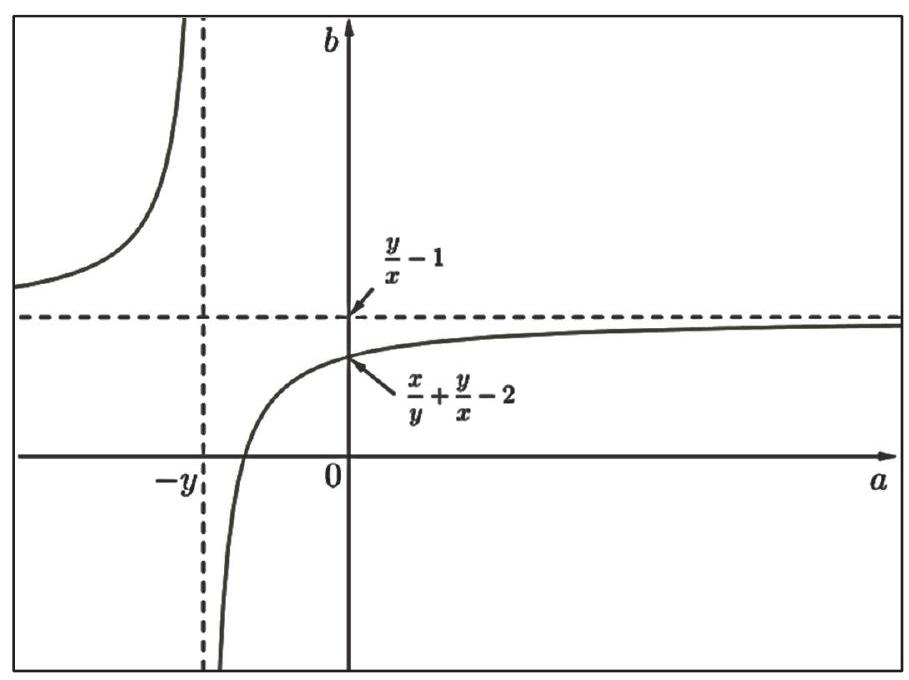
\includegraphics[max width=\textwidth, center]{2025_02_07_d712b9a47aa2c64928dbg-13}

Wynika stąd, że w przedziale $(-y,+\infty)$ funkcja $f$ jest rosnąca. W szczególności jest ona rosnąca w przedziale $\langle 0,+\infty)$. Zatem dla każdego argumentu $a>0$ prawdziwa jest nierówność $f(a)>f(0)$. Zauważmy, że $f(0)=\frac{x+0}{y+0}+\frac{y}{x}-2=\frac{x}{y}+\frac{y}{x}-2>2-2=0$, gdyż liczby $\frac{x}{y} \mathrm{i} \frac{y}{x}$ są dodatnie, różne od 1 i jedna z nich jest odwrotnością drugiej.\\
W efekcie dla każdego argumentu $a>0$ prawdziwa jest nierówność

$$
f(a)=\frac{x+a}{y+a}+\frac{y}{x}-2>0,
$$

czyli

$$
\frac{x+a}{y+a}+\frac{y}{x}>2 .
$$

\section*{V sposób}
Nierówność $\frac{x+a}{y+a}+\frac{y}{x}>2$ możemy przekształcić w sposób równoważny mnożąc obustronnie przez $x(y+a)$, bo z założenia $x(y+a)$ jest większe od zera. Otrzymujemy

$$
x(x+a)+y(y+a)>2 x(y+a)
$$

Przekształcamy otrzymaną nierówność

$$
\begin{gathered}
x^{2}+x a+y^{2}+y a>2 x y+2 x a, \\
x^{2}-2 x y+y^{2}>x a-y a, \\
x^{2}-2 x y+y^{2}>a(x-y), \\
(x-y)^{2}>a(x-y) .
\end{gathered}
$$

Z założenia $x\langle y$ i $a\rangle 0$, zatem $a(x-y)<0$, natomiast kwadrat $(x-y)^{2}$ jest dodatni. W rezultacie otrzymana nierówność jest prawdziwa. To kończy dowód.

\section*{Zadanie 9. (0-3)}
V. Rozumowanie i argumentacja.

\section*{Schemat punktowania}
\section*{Rozwiązanie petne \\
 Zdający zapisze pełne, poprawne rozumowanie.}
\section*{Pokonanie zasadniczych trudności zadania 2 p.}
\section*{Zdający}
\begin{itemize}
  \item zapisze, że trójkąty $A S M$ i $N L C$ lub trójkąty $M K C$ i $B T N$ są przystające, nie uzasadni tego przystawania i uzasadni tezę\\
albo
  \item zapisze dwie proporcje wynikające z podobieństwa trójkątów pozwalające (wraz z równością $|A P|=|B P|$ ) wyznaczyć zależność między długościami odcinków $S T$ i $A B$, np.: $\frac{p}{x}=\frac{a}{b} \mathrm{i} \frac{|B T|}{b-x}=\frac{a}{b}$\\
albo
  \item zapisze dwie proporcje wynikające z twierdzenia Talesa pozwalające (wraz z równością $|A P|=|B P|$ ) wyznaczyć zależność między długościami odcinków $S T$ i $A B$, np.:\\
$\frac{p}{x}=\frac{a-p}{b-x} \mathrm{i} \frac{a-q}{b-x}=\frac{q}{x}$,\\
albo
  \item zapisze długości odcinków $A B, A S$ i $B T$ w zależności od długości odcinków $x=|A M|$, $y=|M C|$ oraz kąta $\alpha$ w postaci : $|A B|=2(x+y) \cdot \cos \alpha,|A S|=x \cdot \cos \alpha$, $|B T|=y \cdot \cos \alpha$,\\
albo
  \item narysuje odcinek $M Z$ równoległy do $B C$ oraz odcinek $Z N$ lub odcinek $N Z$ równoległy do $A C$ oraz odcinek $M Z$, zapisze, że trójkąty $A M Z$ i $Z B N$ są równoramienne, ale nie uzasadni, że czworokąt $M Z N C$ jest równoległobokiem i poprawnie uzasadni tezę\\
i na tym zakończy lub dalej popełni błędy.
\end{itemize}

\section*{Rozwiązanie, w którym postęp jest wprawdzie niewielki, ale konieczny na drodze do całkowitego rozwiązania zadania \\
 1 p.}
\section*{Zdający}
\begin{itemize}
  \item zapisze, że trójkąty $A S M$ i $N L C$ są przystające lub trójkąty $M K C$ i $B T N$ są przystające albo
  \item zapisze, że trójkąty, np. $A S M$ i $A P C$ są podobne lub zapisze proporcję wynikającą z tego podobieństwa,\\
albo
  \item zapisze proporcję wynikającą z twierdzenia Talesa, np.: $\frac{|A S|}{|A M|}=\frac{|S P|}{|M C|}$,\\
albo
  \item wyznaczy długość odcinka $A B$ w zależności od długości odcinków $x=|A M|, y=|M C|$ oraz kąta $\alpha:|A B|^{2}=(x+y)^{2}+(x+y)^{2}-2 \cdot(x+y) \cdot(x+y) \cdot \cos \left(180^{\circ}-2 \alpha\right)$,\\
albo
  \item zapisze dwie zależności: $\frac{|A S|}{|A M|}=\cos \alpha, \frac{|B T|}{|B N|}=\cos \alpha$,\\
albo
  \item narysuje odcinek $M Z$ równoległy do $B C$ oraz odcinek $Z N$ lub odcinek $N Z$ równoległy do $A C$ oraz odcinek $M Z$\\
i na tym zakończy lub dalej popełni błędy.
\end{itemize}

\section*{Uwagi}
\begin{enumerate}
  \item Za uzasadnienie przystawania trójkątów prostokątnych np.: $A S M$ i $N L C$ uznajemy\\
a) powołanie się na cechę przystawania $k b k$, o ile na rysunku nie występują sprzeczne oznaczenia kątów,\\
b) zaznaczenie na rysunku jednej pary odpowiednich kątów ostrych w tych trójkątach.
  \item W III i IV sposobie rozwiązania nie wymagamy uzasadnienia podobieństwa trójkątów lub powołania się na twierdzenie Talesa.
  \item Jeżeli zdający rozpatrzy tylko szczególny przypadek, w którym punkty $M$ i $N$, są środkami boków $A C$ i $B C$, to otrzymuje $\mathbf{0}$ punktów za całe rozwiązanie.
  \item Jeżeli zdający zakłada, że trójkąt $A B C$ jest równoboczny i korzysta z tego założenia, to za całe rozwiązanie otrzymuje 0 punktów.
  \item Jeżeli zdający przedstawia rozwiązanie, w którym odwołuje się tylko do argumentów pozamatematycznych, np. „przesuwa" punkty $M$ i $N$ po odcinkach $A C$ i $B C$ z tymi samymi szybkościami, to może otrzymać $\mathbf{1}$ punkt za zauważenie, że rzuty prostokątne na prostą $A B$ odcinków równych, z których jeden leży na prostej $A C$, a drugi na prostej $B C$ są równe.
\end{enumerate}

\section*{Przykładowe rozwiązania}
I sposób (,,przystawanie trójkątów - I")\\
Niech $P$ będzie środkiem podstawy $A B$ tego trójkąta. Poprowadźmy przez punkty $M$ i $N$ proste równoległe do podstawy $A B$ trójkąta, a ich punkty przecięcia z prostą $C P$ oznaczmy odpowiednio $K$ i $L$. Oznaczmy też $x=|A M|=|C N|, y=|M C|, p=|A S|, q=|M K|$, jak na rysunku.\\
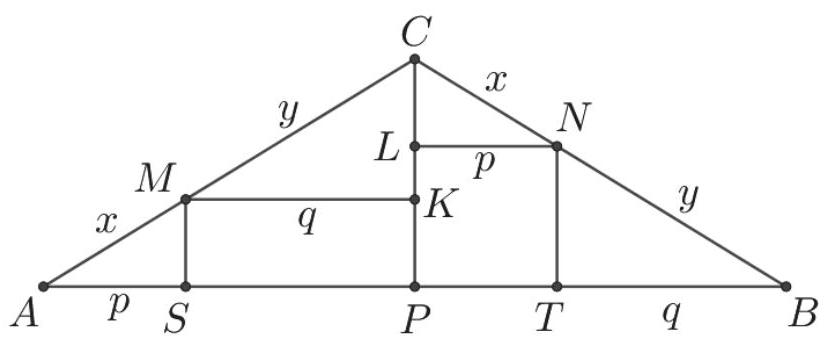
\includegraphics[max width=\textwidth, center]{2025_02_07_d712b9a47aa2c64928dbg-16}

Ponieważ trójkąt $A B C$ jest równoramienny, więc $|N B|=|M C|=y$. Trójkąty $A S M$ i $N L C$ są przystające, gdyż oba są prostokątne, $|A M|=|C N|$ oraz $|\Varangle B A C|=|\Varangle A B C|=|\Varangle L N C|$ oraz $|\Varangle A M S|=90^{\circ}-|\Varangle B A C|=90^{\circ}-|\Varangle L N C|=|\Varangle N C L|$. Podobnie uzasadniamy, że trójkąty $M K C$ i $B T N$ są przystające.\\
Zatem

$$
|P T|=|L N|=|A S|=p \text { oraz }|S P|=|M K|=|T B|=q .
$$

Stąd wynika, że

$$
|S T|=|S P|+|P T|=q+p=\frac{1}{2} \cdot(2 p+2 q)=\frac{1}{2} \cdot|A B| .
$$

II sposób (,„przystawanie trójkątów - II")\\
Niech $P$ będzie środkiem podstawy $A B$ tego trójkąta. Poprowadźmy przez punkt $N$ prostą równoległą do podstawy $A B$ trójkąta, a punkt jej przecięcia z prostą $C P$ oznaczmy przez $L$. Oznaczmy też $x=|A M|=|C N|, p=|A S|$, jak na rysunku.\\
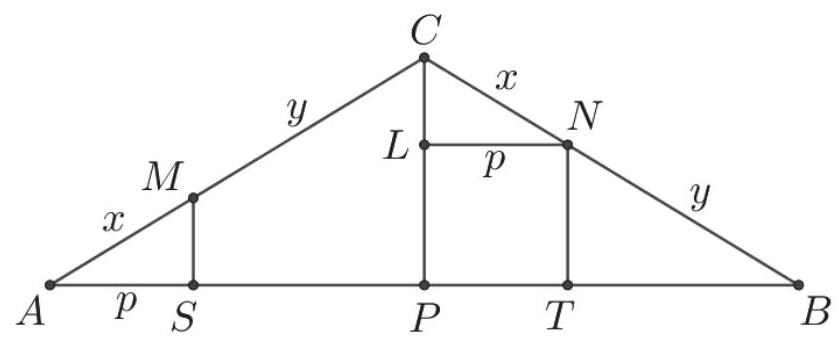
\includegraphics[max width=\textwidth, center]{2025_02_07_d712b9a47aa2c64928dbg-17}

Trójkąty $A S M$ i $N L C$ są przystające, gdyż oba są prostokątne, $|A M|=|C N|$,

$$
|\Varangle B A C|=|\Varangle A B C|=|\Varangle L N C| \text { oraz }|\Varangle A M S|=90^{\circ}-|\Varangle B A C|=90^{\circ}-|\Varangle L N C|=|\Varangle N C L| .
$$

Stąd wynika, że $|P T|=|L N|=|A S|=p$.\\
Ponieważ trójkąt $A B C$ jest równoramienny, więc $|A P|=|B P|$.\\
Stąd wynika, że

$$
|S T|=|S P|+|P T|=(|A P|-p)+p=|A P|=\frac{1}{2} \cdot|A B| .
$$

\section*{Uwaga}
Analogiczne rozumowanie możemy przeprowadzić, wychodząc od pary trójkątów przystających MKC i BTN (oznaczenia jak w I sposobie oceniania).

III sposób („,podobieństwo trójkątów")\\
Niech $P$ będzie środkiem podstawy $A B$ tego trójkąta. Oznaczmy też $x=|A M|=|C N|$, $b=|A C|=|B C|, a=|A P|$, jak na rysunku.\\
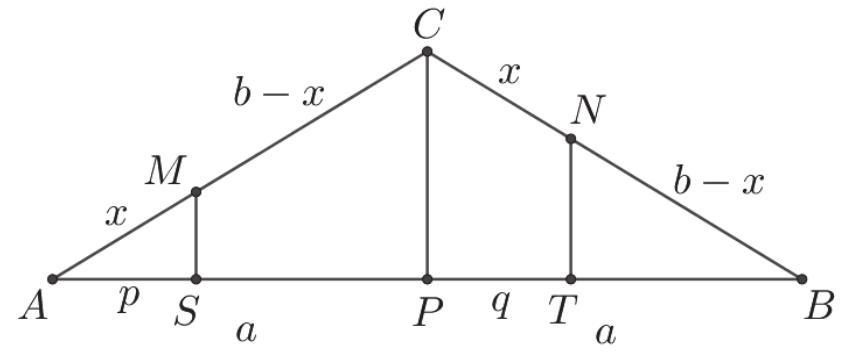
\includegraphics[max width=\textwidth, center]{2025_02_07_d712b9a47aa2c64928dbg-17(1)}

Ponieważ $P$ jest spodkiem wysokości trójkąta równoramiennego, więc $|B P|=|A P|=a$. Trójkąty $A S M$ i $A P C$ są podobne na mocy cechy $k k k$, ponieważ obydwa są trójkątami prostokątnymi (odcinki $S M$ i $P C$ są równoległe), a kąt $P A C$ jest kątem wspólnym obu trójkątów. Stąd wynika, że

$$
\frac{|A S|}{|A M|}=\frac{|A P|}{|A C|}, \operatorname{czyli} \frac{p}{x}=\frac{a}{b} .
$$

Stąd $\quad p=\frac{a x}{b}$. Zatem $|S P|=|A P|-p=a-\frac{a x}{b}$.

Ponieważ $N T \| C P$ i kąt $C B P$ jest kątem wspólnym, więc na mocy cechy kkk trójkąt $B T N$ jest podobny do trójkąta $B P C$. Stąd wynika, że

$$
\frac{|B T|}{|B N|}=\frac{|B P|}{|B C|} \text {, czyli } \frac{|B T|}{b-x}=\frac{a}{b} \text {. }
$$

$\operatorname{Stąd}|B T|=\frac{a(b-x)}{b}$, więc $|P T|=|B P|-|B T|=a-\frac{a(b-x)}{b}=\frac{a b-a b+a x}{b}=\frac{a x}{b}$.\\
Zatem

$$
|S T|=|S P|+|P T|=a-\frac{a x}{b}+\frac{a x}{b}=a=\frac{1}{2} \cdot|A B| .
$$

To kończy dowód.

\section*{IV sposób (,,twierdzenia Talesa")}
Niech $P$ będzie środkiem podstawy $A B$ tego trójkąta. Oznaczmy też $x=|A M|=|C N|$, $b=|A C|=|B C|, a=|A P|, p=|A S|, q=|P T|$, jak na rysunku.\\
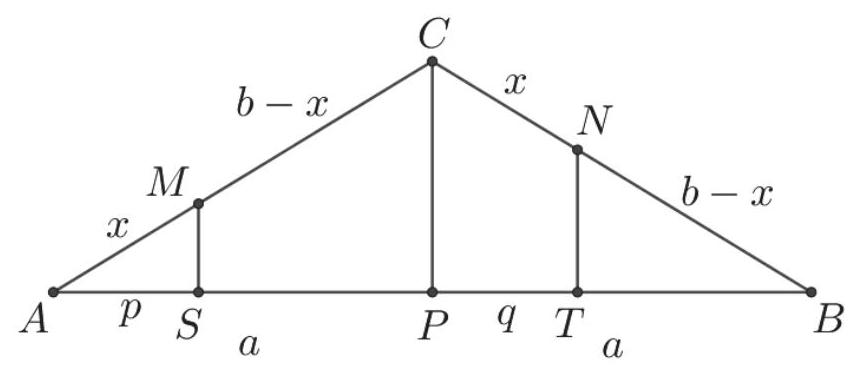
\includegraphics[max width=\textwidth, center]{2025_02_07_d712b9a47aa2c64928dbg-18}

Ponieważ trójkąt $A B C$ jest równoramienny, a $P$ jest spodkiem jego wysokości, więc $|B N|=|M C|=b-x$ i $|B P|=|A P|=a$.\\
Z twierdzenia Talesa otrzymujemy

$$
\frac{|A S|}{|A M|}=\frac{|S P|}{|M C|} \text { oraz } \frac{|B T|}{|B N|}=\frac{|P T|}{|N C|},
$$

czyli

$$
\frac{p}{x}=\frac{a-p}{b-x} \text { oraz } \frac{a-q}{b-x}=\frac{q}{x} .
$$

Stąd

$$
\begin{gathered}
p b-p x=a x-p x \text { oraz } a x-q x=b q-q x, \\
p=\frac{a x}{b} \text { oraz } q=\frac{a x}{b} .
\end{gathered}
$$

Zatem

$$
|S T|=|S P|+|P T|=a-p+q=a-\frac{a x}{b}+\frac{a x}{b}=a=\frac{1}{2} \cdot|A B| .
$$

To kończy dowód.

\section*{V sposób (,"trygonometria")}
Oznaczmy $\alpha=|\Varangle B A C|=|\Varangle A B C|, x=|A M|=|C N|, y=|M C|, 2 a=|A P|$, jak na rysunku.\\
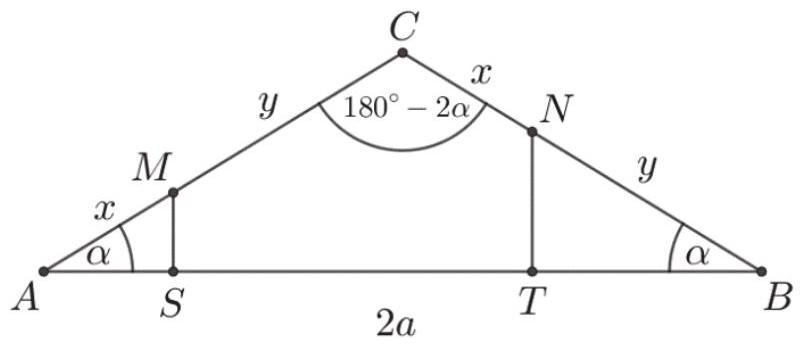
\includegraphics[max width=\textwidth, center]{2025_02_07_d712b9a47aa2c64928dbg-19(1)}

Wtedy $|N B|=|B C|-x=|A C|-x=y$ oraz $|\Varangle A C B|=180^{\circ}-2 \alpha$.\\
Z twierdzenia cosinusów dla trójkąta $A B C$ otrzymujemy

$$
\begin{gathered}
|A B|^{2}=|A C|^{2}+|B C|^{2}-2 \cdot|A C| \cdot|B C| \cdot \cos \left(180^{\circ}-2 \alpha\right), \\
|A B|^{2}=(x+y)^{2}+(x+y)^{2}-2 \cdot(x+y) \cdot(x+y) \cdot \cos \left(180^{\circ}-2 \alpha\right), \\
|A B|^{2}=2(x+y)^{2}+2 \cdot(x+y)^{2} \cdot \cos 2 \alpha, \\
|A B|^{2}=2(x+y)^{2}\left(1+\cos ^{2} \alpha-\sin ^{2} \alpha\right), \\
|A B|^{2}=4(x+y)^{2} \cdot \cos ^{2} \alpha .
\end{gathered}
$$

Stąd

$$
|A B|=2(x+y) \cdot \cos \alpha .
$$

Z trójkątów $A S M$ i $B T N$ otrzymujemy

$$
\begin{aligned}
& \frac{|A S|}{|A M|}=\cos \alpha \text { oraz } \frac{|B T|}{|B N|}=\cos \alpha, \\
& \frac{|A S|}{x}=\cos \alpha \text { oraz } \frac{|B T|}{y}=\cos \alpha
\end{aligned}
$$

Stąd

$$
|A S|=x \cdot \cos \alpha \text { oraz }|B T|=y \cdot \cos \alpha .
$$

Zatem\\
$|S T|=|A B|-|A S|-|B T|=2(x+y) \cdot \cos \alpha-x \cdot \cos \alpha-y \cdot \cos \alpha=(x+y) \cdot \cos \alpha=\frac{1}{2} \cdot|A B|$.\\
To kończy dowód.

VI sposób („trójkąty równoramienne")\\
Narysujmy odcinek $M Z$ równoległy do prostej $B C$ taki, że koniec $Z$ tego odcinka leży na podstawie $A B$ trójkąta $A B C$ oraz odcinek $N Z$. Oznaczmy też $x=|A M|=|C N|, \quad y=|M C|$, $p=|A S|, q=|T B|$, jak na rysunku.\\
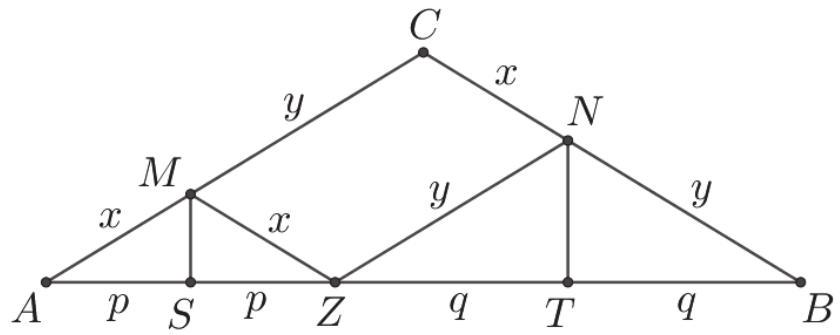
\includegraphics[max width=\textwidth, center]{2025_02_07_d712b9a47aa2c64928dbg-19}

Wtedy kąty odpowiadające $A Z M$ i $A B C$ są równe. To oznacza, że trójkąt $A Z M$ jest równoramienny. Stąd wynika, że $|M Z|=|A M|=|C N|=x$. Zatem czworokąt MZNC jest równoległobokiem (jego boki $M Z$ i $C N$ są równoległe i mają równe długości), co oznacza, że $|Z N|=|M C|=y$. To z kolei oznacza, że trójkąt $Z B N$ jest równoramienny. Punkty $S$ i $T$ to spodki wysokości trójkątów równoramiennych, więc

$$
|A S|=|S Z|=p \text { oraz }|Z T|=|T B|=q .
$$

Stąd

$$
|S T|=|S P|+|P T|=q+p=\frac{1}{2} \cdot(2 p+2 q)=\frac{1}{2} \cdot|A B| .
$$

To kończy dowód.\\
IV. Użycie i tworzenie strategii.\\
7. Planimetria. Zdający znajduje związki miarowe w figurach płaskich z zastosowaniem twierdzenia sinusów i twierdzenia cosinusów (R7.5).

\section*{Schemat punktowania}
\section*{Rozwiązanie pelne}
4 p.\\
Zdający obliczy obwód trójkąta $A B C: L_{A B C}=120$.

Pokonanie zasadniczych trudności zadania\\
3 p.\\
Zdający zapisze równanie wymierne z jedną niewiadomą $a$, np.:\\
$a^{2}=256+a^{2}+12 a+36-2 \cdot 16 \cdot(a+6) \cdot \frac{1}{2} \quad$ lub $\quad a^{2}=\frac{49}{\left(\frac{1}{7}\right)^{2}}, \quad$ lub $\quad \frac{1}{7}=\frac{7}{a}, \quad$ lub $a^{2}=(8 \sqrt{3})^{2}+(a-2)^{2}$, lub $a^{2}=(\sqrt{192})^{2}+(a-2)^{2}$, lub $16^{2} \cdot a+a^{2} \cdot 6=(a+6)\left(14^{2}+a \cdot 6\right)$, lub $48 a^{2}=49\left(a^{2}-49\right)$, lub $49\left(1-\frac{49}{a^{2}}\right)=48$, lub $\frac{a}{\frac{4 \sqrt{3}}{7}}=\frac{14}{2 \cdot \frac{4 \sqrt{3}}{7} \cdot \frac{1}{7}} \quad$, lub $\frac{a}{14}=\frac{7}{2}$, lub\\
$16^{2}=(a+6)^{2}+a^{2}-2 \cdot(a+6) \cdot a \cdot \frac{2 a^{2}-14^{2}}{2 a^{2}}$, lub $(a+11)(a-5) \cdot 5 \cdot 11=(24 \sqrt{3}+4 \sqrt{3} \cdot a)^{2}$.

Rozwiązanie, w którym jest istotny postęp 2 p.\\
Zdający

\begin{itemize}
  \item obliczy $\cos \alpha=\frac{1}{2}$ oraz zapisze równanie wynikające $z$ twierdzenia cosinusów dla trójkąta $A B C: a^{2}=16^{2}+(a+6)^{2}-2 \cdot 16 \cdot(a+6) \cdot \cos \alpha$\\
albo
  \item obliczy $\cos \omega=\frac{1}{7}$ oraz zapisze równanie wynikające $z$ twierdzenia cosinusów dla trójkąta $B C D$, np.: $14^{2}=a^{2}+a^{2}-2 \cdot a \cdot a \cdot \cos \left(180^{\circ}-2 \omega\right)$ lub $a^{2}=a^{2}+14^{2}-2 \cdot 14 a \cdot \cos \omega$,\\
albo
  \item obliczy $\sin \omega=\frac{4 \sqrt{3}}{7}$ oraz $\sin \left(180^{\circ}-2 \omega\right)=2 \cdot 4 \frac{\sqrt{3}}{7} \cdot \frac{1}{7}$,\\
albo
  \item obliczy $\cos \omega=\frac{1}{7}$ oraz zapisze równanie wynikające $z$ definicji cosinusa w trójkącie $B C D: \cos \omega=\frac{|E D|}{a}$,\\
albo
  \item obliczy $|A F|=8,|C F|=8 \sqrt{3}$ oraz wyznaczy długość odcinka $B F$ w zależności od $a$ : $|B F|=a-2$,\\
albo
  \item obliczy pole trójkąta $A D C$, wyznaczy pole trójkąta $B C D$ w zależności od $a$ oraz wyznaczy stosunek pól trójkątów $A D C$ i $B C D$ w zależności od $a: P_{A D C}=24 \sqrt{3}$, $P_{B C D}=7 \sqrt{a^{2}-49}, \frac{P_{A D C}}{P_{B C D}}=\frac{6}{a}$,\\
albo
  \item zapisze równanie pierwiastkowe z niewiadomą $a: a=\frac{4 \sqrt{3}}{\frac{7}{a} \sqrt{1-\frac{49}{a^{2}}}}$,\\
albo
  \item obliczy pole trójkąta $A D C$, wysokość $C F$ oraz długość odcinka $D F: P_{A D C}=24 \sqrt{3}$, $|C F|=8 \sqrt{3},|D F|=2$,\\
albo
  \item zapisze układ równań z dwiema niewiadomymi $a \mathrm{i} \cos \beta$ : $16^{2}=(a+6)^{2}+a^{2}-2 \cdot(a+6) \cdot a \cdot \cos \beta$ i $14^{2}=a^{2}+a^{2}-2 \cdot a \cdot a \cdot \cos \beta$,\\
albo
  \item obliczy pole trójkąta $A D C$ oraz wyznaczy pola trójkątów $A B C$ i $B C D$ w zależności od $a$ :
\end{itemize}

$$
P_{A D C}=24 \sqrt{3}, P_{A B C}=\sqrt{(a+11)(a-5) \cdot 5 \cdot 11}, P_{B C D}=\frac{1}{2} \cdot 8 \sqrt{3} \cdot a
$$

i na tym zakończy lub dalej popełnia błędy.

\section*{Rozwiązanie, w którym postęp jest niewielki, ale konieczny na drodze do pełnego rozwiązania zadania}
Zdający

\begin{itemize}
  \item obliczy $\cos \alpha=\frac{1}{2}$\\
albo
  \item zapisze równanie wynikające z twierdzenia cosinusów dla trójkąta $A B C$ : $a^{2}=16^{2}+(a+6)^{2}-2 \cdot 16 \cdot(a+6) \cdot \cos \alpha$ lub $16^{2}=(a+6)^{2}+a^{2}-2 \cdot(a+6) \cdot a \cdot \cos \beta$,\\
albo
  \item obliczy $\cos \delta=-\frac{1}{7}$ lub $\cos \omega=\frac{1}{7}$,\\
albo
  \item zapisze, że $\cos \omega=\frac{|E D|}{a}$ lub $\cos \omega=\frac{7}{a}$,\\
albo
  \item zapisze układ dwóch równań z dwiema niewiadomymi:
\end{itemize}

$$
16^{2}=h^{2}+(x+6)^{2} \text { oraz } 14^{2}=h^{2}+x^{2}
$$

albo

\begin{itemize}
  \item obliczy pole trójkąta $A D C$ i wyznaczy pole trójkąta $B C D$ w zależności od $a$ - długości boku $B C$ : $P_{A D C}=24 \sqrt{3}, \quad P_{B C D}=7 \sqrt{a^{2}-49}$,\\
albo
  \item obliczy pole trójkąta $A D C$ i wyznaczy pola trójkątów $A B C$ i $B C D$ w zależności od $a$ długości boku $B C$ oraz $\sin \beta: P_{A D C}=24 \sqrt{3}, P_{A B C}=\frac{1}{2} \cdot(a+6) \cdot a \cdot \sin \beta$,
\end{itemize}

$$
P_{B C D}=\frac{1}{2} \cdot a \cdot a \cdot \sin \beta,
$$

albo

\begin{itemize}
  \item obliczy pole trójkąta $A D C$ oraz wysokość $C F: P_{A D C}=24 \sqrt{3},|C F|=8 \sqrt{3}$,\\
albo
  \item zapisze równanie wynikające z twierdzenia cosinusów dla trójkąta $B C D$ :\\
$14^{2}=a^{2}+a^{2}-2 \cdot a \cdot a \cdot \cos \beta$\\
i na tym zakończy lub dalej popełnia błędy.
\end{itemize}

\section*{Uwagi}
\begin{enumerate}
  \item Jeżeli zdający realizuje strategię rozwiązania i popełnia jedynie błędy rachunkowe, to może otrzymać 3 punkty, o ile popełnione błędy nie ułatwiają rozważanego zagadnienia na żadnym etapie rozwiązania.
  \item Jeżeli zdający pominie współczynnik $\frac{1}{2}$ we wzorze na pole trójkąta, to może otrzymać 3 punkty za rozwiązanie zadania konsekwentnie do końca.
  \item Jeżeli zdający realizuje strategię rozwiązania i jedynym błędem, który jednak nie ułatwia rozważania zagadnienia na żadnym etapie rozwiązania, jest błąd, polegający na niepoprawnym zastosowaniu:\\
a) twierdzenia cosinusów lub twierdzenia sinusów, lub niewłaściwym podstawieniu do wzoru z tego twierdzenia,\\
b) definicji funkcji trygonometrycznej,\\
c) wzoru Herona,\\
d) twierdzenia Pitagorasa,\\
e) wzoru redukcyjnego,\\
f) wzoru na pole trójkąta $z$ sinusem kąta między bokami,\\
g) twierdzenia Stewarta,\\
h) wzoru , $\sqrt{a^{2}-b^{2}}=\sqrt{a^{2}}-\sqrt{b^{2}}$ " lub , $(a+b)^{2}=a^{2}+b^{2}$,,\\
to zdający otrzymuje co najwyżej 2 punkty za rozwiązanie całego zadania.
  \item Jeżeli zdający realizuje strategię rozwiązania, i popełnia jeden błąd, wymieniony w uwadze 3., a ponadto popełnia błędy rachunkowe, to otrzymuje $\mathbf{1}$ punkt.
  \item Jeżeli zdający stosuje przybliżenia funkcji trygonometrycznych i tym samym zmienia aspekt rozważanego zagadnienia, to może otrzymać co najwyżej $\mathbf{3}$ punkty za całe rozwiązanie.
  \item Jeżeli zdający zakłada, że kąt $C A D$ ma miarę 60 stopni, to może uzyskać jedynie punkty za te części rozwiązania, w których nie korzysta z tego nieuprawnionego założenia.
\end{enumerate}

\section*{Przykładowe rozwiązania}
I sposób\\
Przyjmijmy oznaczenia jak na rysunku.\\
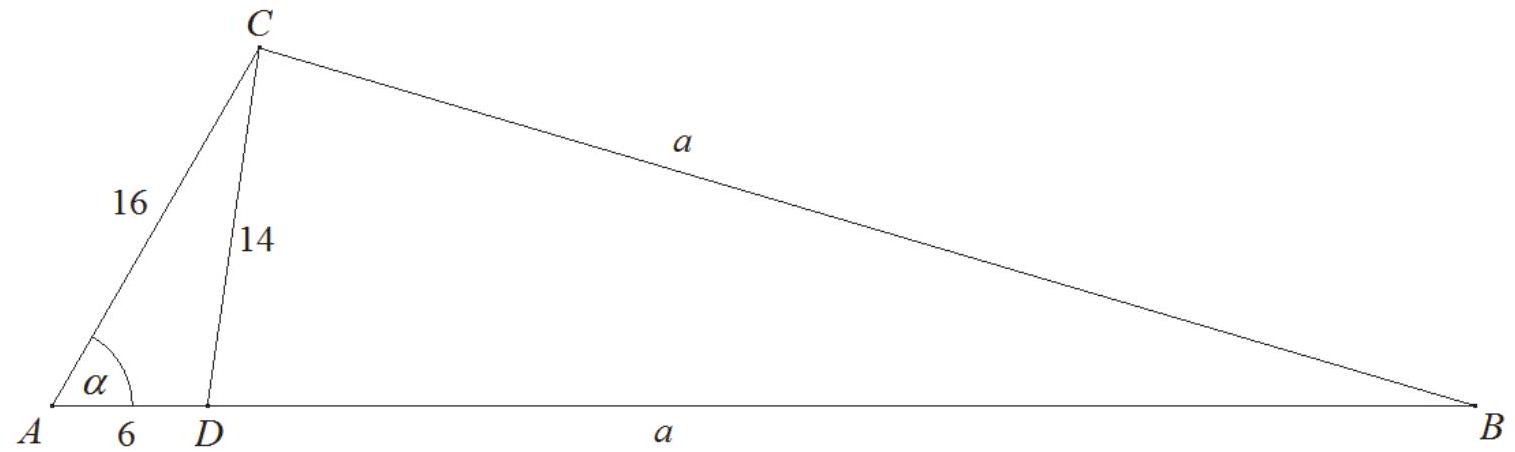
\includegraphics[max width=\textwidth, center]{2025_02_07_d712b9a47aa2c64928dbg-24(1)}

Z twierdzenia cosinusów dla trójkąta $A D C$ otrzymujemy

$$
14^{2}=16^{2}+6^{2}-2 \cdot 16 \cdot 6 \cdot \cos \alpha .
$$

Stąd

$$
\cos \alpha=\frac{16^{2}+6^{2}-14^{2}}{2 \cdot 16 \cdot 6}=\frac{1}{2} .
$$

Zatem $\alpha=60^{\circ}$.\\
Z twierdzenia cosinusów dla trójkąta $A B C$ otrzymujemy

$$
\begin{gathered}
a^{2}=16^{2}+(a+6)^{2}-2 \cdot 16 \cdot(a+6) \cdot \cos \alpha, \\
a^{2}=256+a^{2}+12 a+36-2 \cdot 16 \cdot(a+6) \cdot \frac{1}{2}, \\
4 a=196, \\
a=49 .
\end{gathered}
$$

Obwód trójkąta $A B C$ jest równy

$$
L_{A B C}=16+6+2 \cdot 49=120 .
$$

II sposób\\
Przyjmijmy oznaczenia jak na rysunku.\\
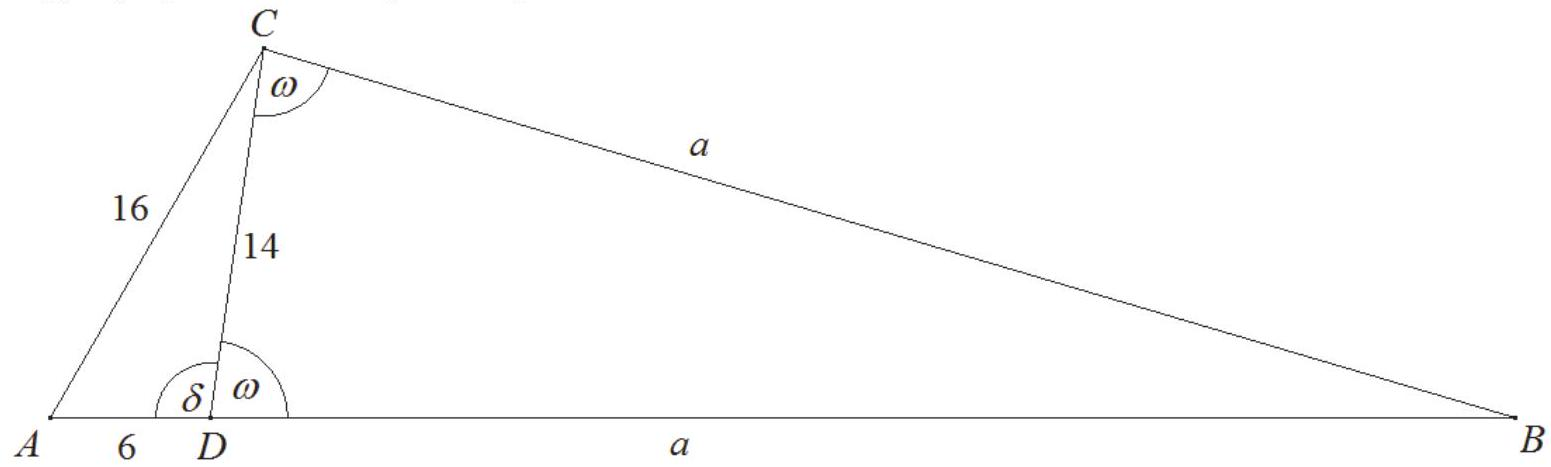
\includegraphics[max width=\textwidth, center]{2025_02_07_d712b9a47aa2c64928dbg-24}

Z twierdzenia cosinusów dla trójkąta $A D C$ otrzymujemy

$$
16^{2}=14^{2}+6^{2}-2 \cdot 14 \cdot 6 \cdot \cos \delta .
$$

Stąd

$$
\cos \delta=\frac{14^{2}+6^{2}-16^{2}}{2 \cdot 14 \cdot 6}=-\frac{1}{7} .
$$

Zatem

$$
\cos \omega=\cos \left(180^{\circ}-\delta\right)=-\cos \delta=-\left(-\frac{1}{7}\right)=\frac{1}{7}
$$

Z twierdzenia cosinusów dla trójkąta $B C D$ otrzymujemy

$$
\begin{gathered}
14^{2}=a^{2}+a^{2}-2 \cdot a \cdot a \cdot \cos \left(180^{\circ}-2 \omega\right), \\
196=2 a^{2}(1+\cos 2 \omega), \\
a^{2}=\frac{98}{1+\cos 2 \omega}=\frac{98}{1+2 \cos ^{2} \omega-1}=\frac{49}{\cos ^{2} \omega}=\frac{49}{\left(\frac{1}{7}\right)^{2}}=49^{2}, a=49
\end{gathered}
$$

albo

$$
\begin{gathered}
a^{2}=a^{2}+14^{2}-2 \cdot 14 a \cdot \cos \omega, \\
28 a \cdot \frac{1}{7}=196, a=49,
\end{gathered}
$$

albo z twierdzenia sinusów otrzymujemy

$$
\begin{aligned}
\frac{a}{\sin \omega} & =\frac{14}{\sin \left(180^{\circ}-2 \omega\right)} \\
\sin \left(180^{\circ}-2 \omega\right) & =\sin 2 \omega=2 \sin \omega \cdot \cos \omega \\
\sin \left(180^{\circ}-2 \omega\right) & =2 \cdot \frac{4 \sqrt{27}}{21} \cdot \frac{3}{21}=\frac{24 \sqrt{27}}{441} \\
\frac{a}{\frac{4 \sqrt{27}}{21}} & =\frac{14}{2 \cdot \frac{4 \sqrt{27}}{21} \cdot \frac{3}{21}} \\
a & =\frac{14}{\frac{6}{21}}=49 .
\end{aligned}
$$

Więc obwód trójkąta $A B C$ jest równy

$$
L_{A B C}=16+6+2 \cdot 49=120 .
$$

\section*{III sposób}
Przyjmijmy oznaczenia jak na rysunku.\\
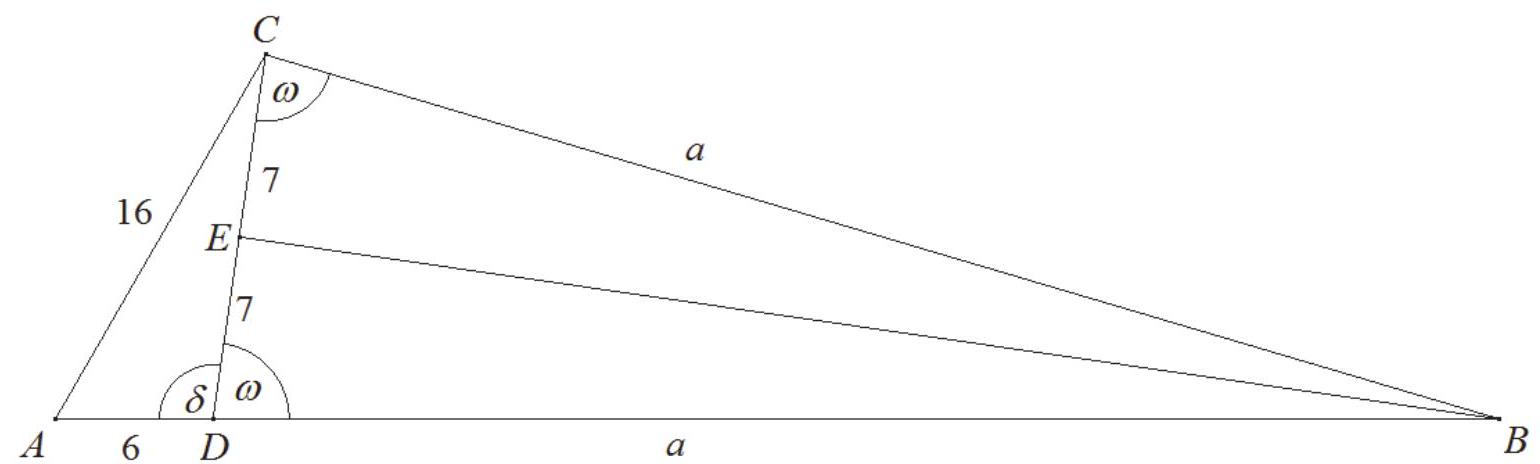
\includegraphics[max width=\textwidth, center]{2025_02_07_d712b9a47aa2c64928dbg-26(1)}

Z twierdzenia cosinusów dla trójkąta $A D C$ otrzymujemy

$$
16^{2}=14^{2}+6^{2}-2 \cdot 14 \cdot 6 \cdot \cos \delta
$$

Stąd

$$
\cos \delta=\frac{14^{2}+6^{2}-16^{2}}{2 \cdot 14 \cdot 6}=-\frac{1}{7}
$$

Zatem

$$
\cos \omega=\cos \left(180^{\circ}-\delta\right)=-\cos \delta=-\left(-\frac{1}{7}\right)=\frac{1}{7} .
$$

Trójkąt $B C D$ jest równoramienny, więc spodek $E$ wysokości $B E$ tego trójkąta jest środkiem boku $C D$. Zatem

$$
\begin{aligned}
\cos \omega & =\frac{|E D|}{a}, \\
\frac{1}{7} & =\frac{7}{a}
\end{aligned}
$$

Stąd $a=49$, więc obwód trójkąta $A B C$ jest równy

$$
L_{A B C}=16+6+2 \cdot 49=120 .
$$

IV sposób\\
Poprowadźmy wysokość $C F$ trójkąta $A B C$ i przyjmijmy oznaczenia jak na rysunku.\\
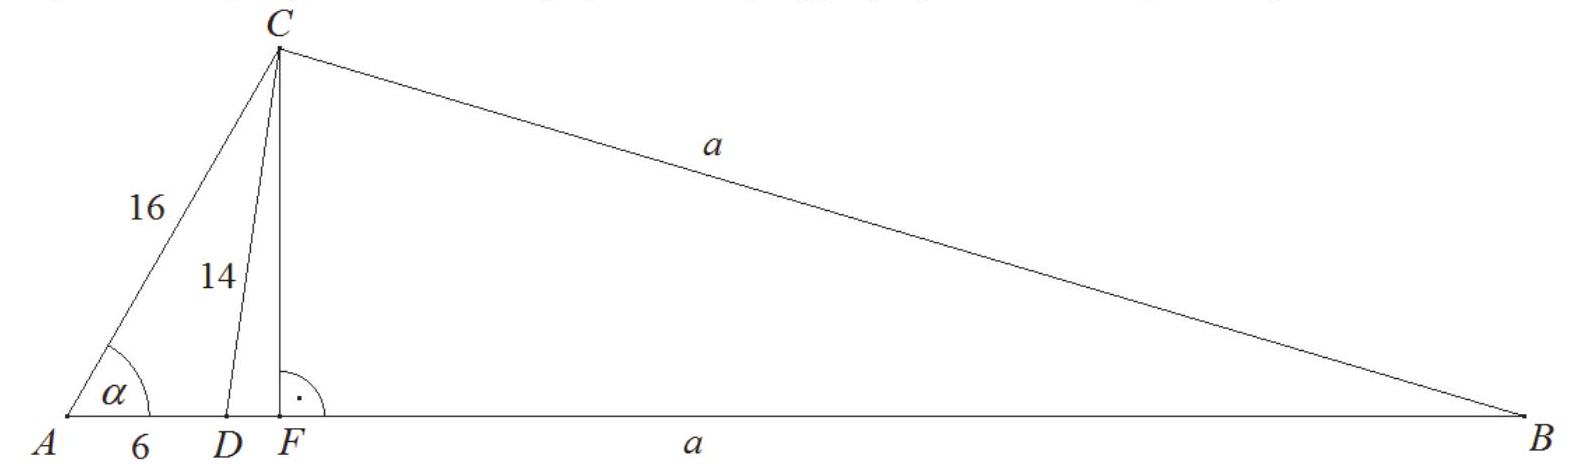
\includegraphics[max width=\textwidth, center]{2025_02_07_d712b9a47aa2c64928dbg-26}

Z twierdzenia cosinusów dla trójkąta $A D C$ otrzymujemy

$$
14^{2}=16^{2}+6^{2}-2 \cdot 16 \cdot 6 \cdot \cos \alpha .
$$

Stąd

$$
\cos \alpha=\frac{16^{2}+6^{2}-14^{2}}{2 \cdot 16 \cdot 6}=\frac{1}{2} .
$$

Zatem $\alpha=60^{\circ}$. Trójkąt $A F C$ jest więc połową trójkąta równobocznego o boku długości 16 . Stąd $|A F|=8$ i $|C F|=8 \sqrt{3}$.

W rezultacie $|D F|=|A F|-|A D|=8-6=2$ oraz $|B F|=|B D|-|D F|=a-2$.\\
Z twierdzenia Pitagorasa dla trójkąta $B C F$ otrzymujemy

$$
\begin{gathered}
a^{2}=(8 \sqrt{3})^{2}+(a-2)^{2}, \\
a^{2}=192+a^{2}-4 a+4 \\
4 a=196, \\
a=49 .
\end{gathered}
$$

Obwód trójkąta $A B C$ jest równy

$$
L_{A B C}=16+6+2 \cdot 49=120 .
$$

V sposób\\
Poprowadźmy wysokość $C F$ trójkąta $A B C$ i przyjmijmy oznaczenia jak na rysunku.\\
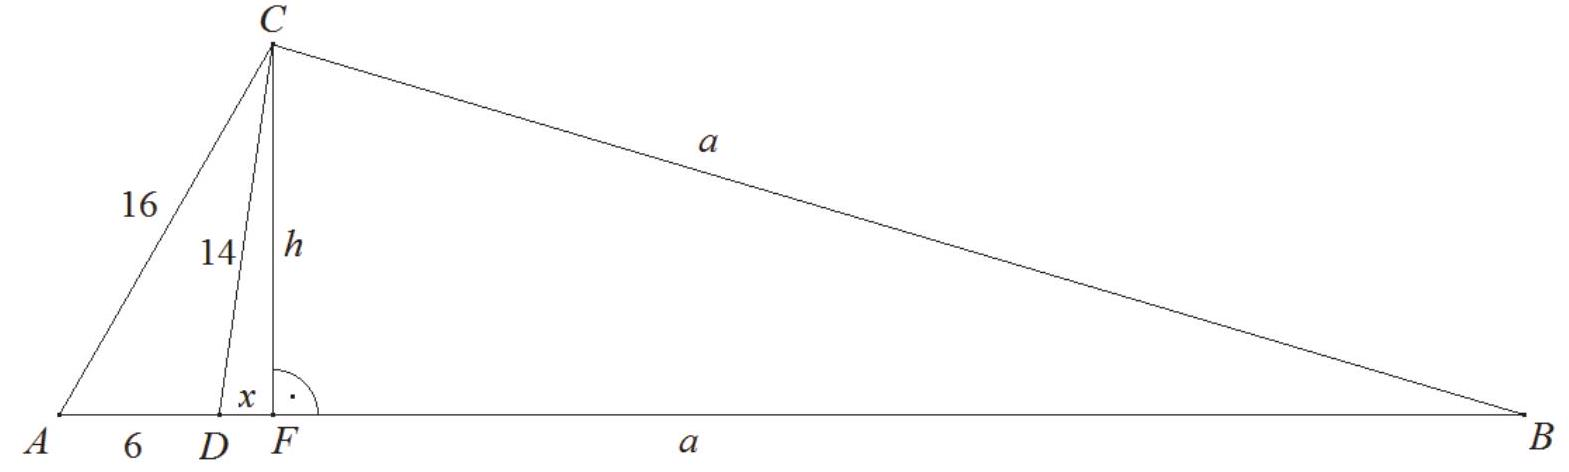
\includegraphics[max width=\textwidth, center]{2025_02_07_d712b9a47aa2c64928dbg-27}

Z twierdzenia Pitagorasa dla trójkątów $A F C$ i $D F C$ otrzymujemy

$$
\begin{gathered}
16^{2}=h^{2}+(x+6)^{2} \text { oraz } 14^{2}=h^{2}+x^{2}, \\
256=h^{2}+x^{2}+12 x+36 \text { oraz } 196=h^{2}+x^{2}, \\
220=196+12 x \text { oraz } h^{2}=196-x^{2}, \\
24=12 x \text { oraz } h^{2}=196-x^{2} \\
x=2 \text { oraz } h=\sqrt{196-2^{2}}=\sqrt{192} .
\end{gathered}
$$

Zatem $|B F|=|B D|-|D F|=a-2$.\\
Z twierdzenia Pitagorasa dla trójkąta $B C F$ otrzymujemy

$$
\begin{gathered}
a^{2}=(\sqrt{192})^{2}+(a-2)^{2}, \\
a^{2}=192+a^{2}-4 a+4 \\
4 a=196, \\
a=49 .
\end{gathered}
$$

Obwód trójkąta $A B C$ jest równy

$$
L_{A B C}=16+6+2 \cdot 49=120 .
$$

\section*{VI sposób}
Przyjmijmy oznaczenia jak na rysunku.\\
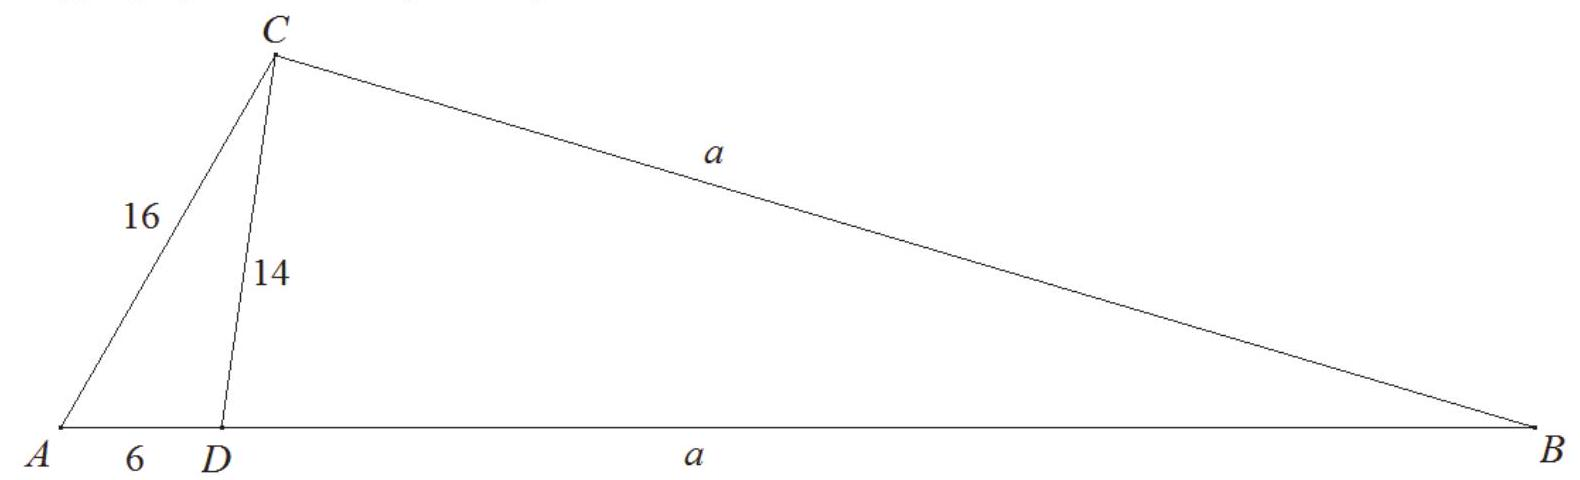
\includegraphics[max width=\textwidth, center]{2025_02_07_d712b9a47aa2c64928dbg-28(1)}

Z twierdzenia Stewarta dla trójkąta $A B C$ otrzymujemy

$$
\begin{gathered}
16^{2} \cdot a+a^{2} \cdot 6=(a+6)\left(14^{2}+a \cdot 6\right) \\
6 a^{2}+256 a=(a+6)(6 a+196), \\
3 a^{2}+128 a=3 a^{2}+116 a+588 \\
12 a=588 \\
a=49
\end{gathered}
$$

Obwód trójkąta $A B C$ jest równy

$$
L_{A B C}=16+6+2 \cdot 49=120 .
$$

VII sposób\\
Przyjmijmy oznaczenia jak na rysunku.\\
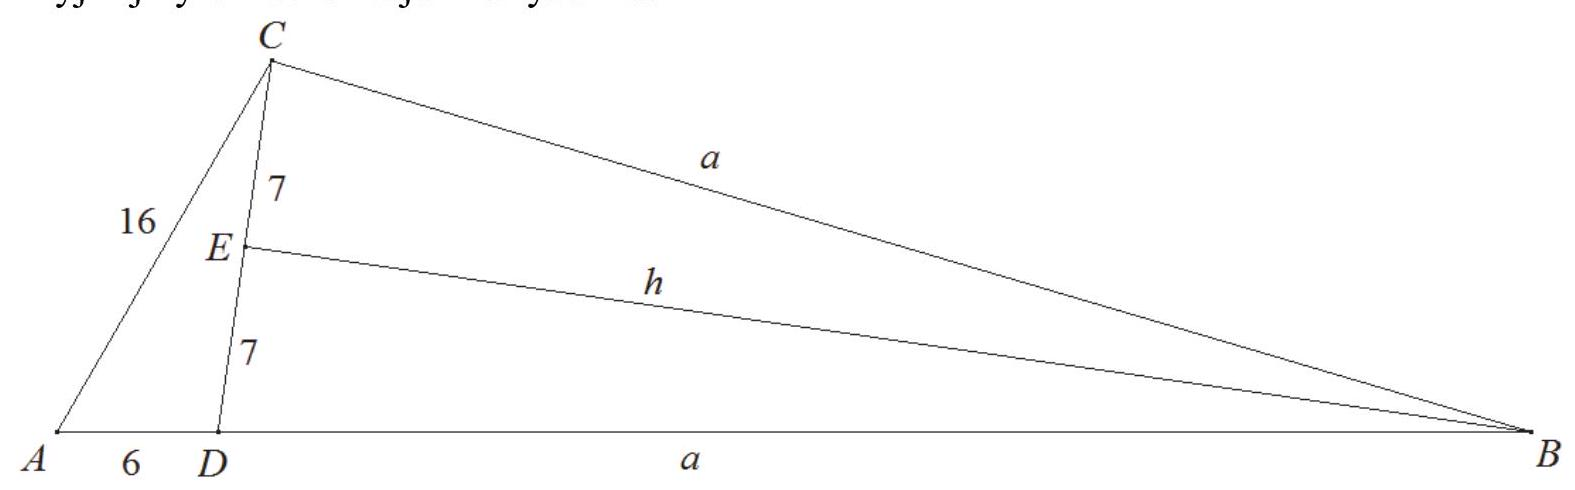
\includegraphics[max width=\textwidth, center]{2025_02_07_d712b9a47aa2c64928dbg-28}

Obliczmy pole trójkąta $A D C$ ze wzoru Herona.\\
Połowa obwodu tego trójkąta jest równa $p=\frac{16+14+6}{2}=18$, więc

$$
P_{A D C}=\sqrt{18 \cdot(18-16) \cdot(18-14) \cdot(18-6)}=\sqrt{18 \cdot 2 \cdot 4 \cdot 12}=24 \sqrt{3} .
$$

Trójkąt $B C D$ jest równoramienny, więc wysokość $h$ opuszczona na bok $C D$ jest równa

$$
h=\sqrt{a^{2}-7^{2}}=\sqrt{a^{2}-49} .
$$

Zatem

$$
P_{B C D}=\frac{1}{2} \cdot 14 \sqrt{a^{2}-49}=7 \sqrt{a^{2}-49} .
$$

Ponieważ trójkąty $A D C$ i $B C D$ mają wspólną wysokość opuszczoną z wierzchołka $C$, więc

$$
\frac{P_{A D C}}{P_{B C D}}=\frac{6}{a},
$$

czyli

$$
\begin{gathered}
\frac{24 \sqrt{3}}{7 \sqrt{a^{2}-49}}=\frac{6}{a} \\
4 a \sqrt{3}=7 \sqrt{a^{2}-49} .
\end{gathered}
$$

Stąd

$$
\begin{gathered}
48 a^{2}=49\left(a^{2}-49\right), \\
48 a^{2}=49 a^{2}-49^{2}, \\
a^{2}=49^{2} .
\end{gathered}
$$

Zatem

$$
a=49 .
$$

Obwód trójkąta $A B C$ jest równy

$$
L_{A B C}=16+6+2 \cdot 49=120 .
$$

\section*{VIII sposób}
Przyjmijmy oznaczenia jak na rysunku.\\
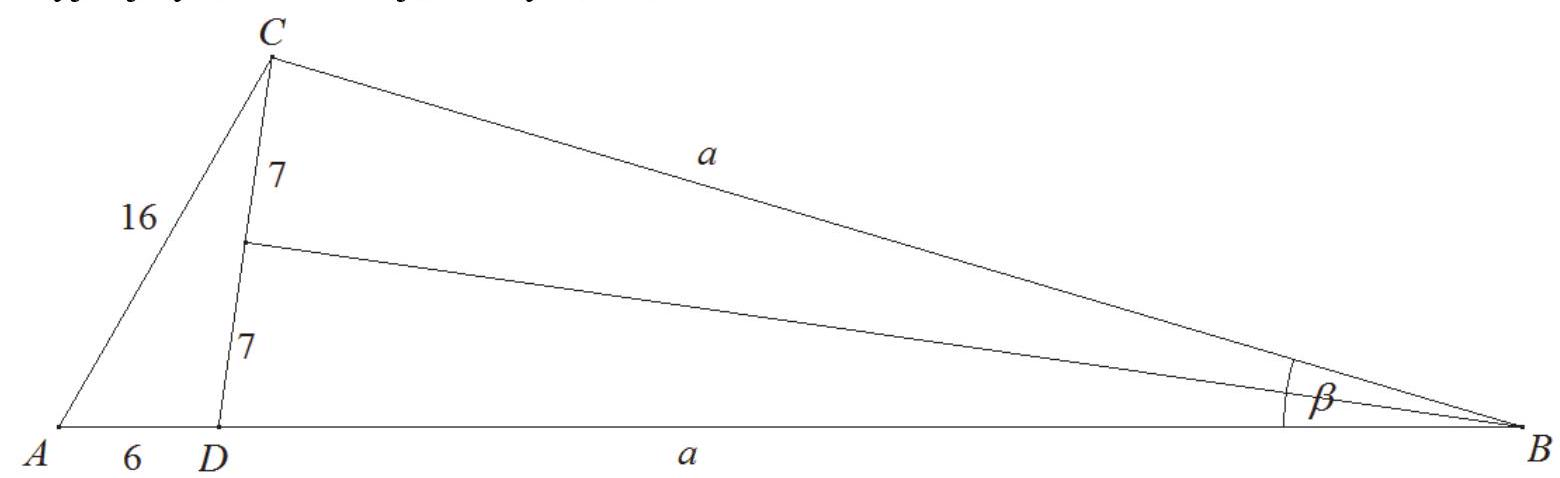
\includegraphics[max width=\textwidth, center]{2025_02_07_d712b9a47aa2c64928dbg-29}

Obliczmy pole trójkąta $A D C$ ze wzoru Herona.\\
Połowa obwodu tego trójkąta jest równa $p=\frac{16+14+6}{2}=18$, więc

$$
P_{A D C}=\sqrt{18 \cdot(18-16) \cdot(18-14) \cdot(18-6)}=\sqrt{18 \cdot 2 \cdot 4 \cdot 12}=24 \sqrt{3} .
$$

Pola trójkątów $A B C$ i $B C D$ są równe odpowiednio

$$
P_{A B C}=\frac{1}{2} \cdot(a+6) \cdot a \cdot \sin \beta \text { oraz } P_{B C D}=\frac{1}{2} \cdot a \cdot a \cdot \sin \beta .
$$

Ponieważ, $P_{A B C}=P_{B D C}+P_{A D C}$, więc

$$
\begin{gathered}
\frac{1}{2} \cdot(a+6) \cdot a \cdot \sin \beta=\frac{1}{2} \cdot a^{2} \cdot \sin \beta+24 \sqrt{3}, \\
a^{2} \sin \beta+6 a \sin \beta=a^{2} \sin \beta+48 \sqrt{3}, \\
a \sin \beta=8 \sqrt{3}, \\
a=\frac{8 \sqrt{3}}{\sin \beta} \\
a=\frac{8 \sqrt{3}}{2 \sin \frac{\beta}{2} \cos \frac{\beta}{2}} \\
a=\frac{4 \sqrt{3}}{\sin \frac{\beta}{2} \cos \frac{\beta}{2}} .
\end{gathered}
$$

(1)

Ponieważ trójkąt $B C D$ jest równoramienny, więc wysokość opuszczona na podstawę $C D$ dzieli ten trójkąt na dwa przystające trójkąty prostokątne. Zatem


\begin{equation*}
\sin \frac{\beta}{2}=\frac{7}{a} . \tag{2}
\end{equation*}


Z jedynki trygonometrycznej otrzymujemy\\
(3)

$$
\cos \frac{\beta}{2}=\sqrt{1-\sin ^{2} \frac{\beta}{2}}=\sqrt{1-\frac{49}{a^{2}}} .
$$

Z (1), (2) i (3) otrzymujemy równanie z niewiadomą $a$

$$
a=\frac{4 \sqrt{3}}{\frac{7}{a} \sqrt{1-\frac{49}{a^{2}}}} .
$$

Stąd

$$
\begin{gathered}
a \cdot \frac{7}{a} \sqrt{1-\frac{49}{a^{2}}}=4 \sqrt{3}, \\
7 \sqrt{1-\frac{49}{a^{2}}}=4 \sqrt{3}, \\
49\left(1-\frac{49}{a^{2}}\right)=48, \\
49-\frac{49^{2}}{a^{2}}=48, \\
1=\frac{49^{2}}{a^{2}}, \\
a^{2}=49^{2} .
\end{gathered}
$$

Zatem

$$
a=49 .
$$

Obwód trójkąta $A B C$ jest równy

$$
L_{A B C}=16+6+2 \cdot 49=120 .
$$

\section*{IX sposób}
Poprowadźmy wysokości $C F$ i $B E$ trójkąta $B C D$ i przyjmijmy oznaczenia jak na rysunku.\\
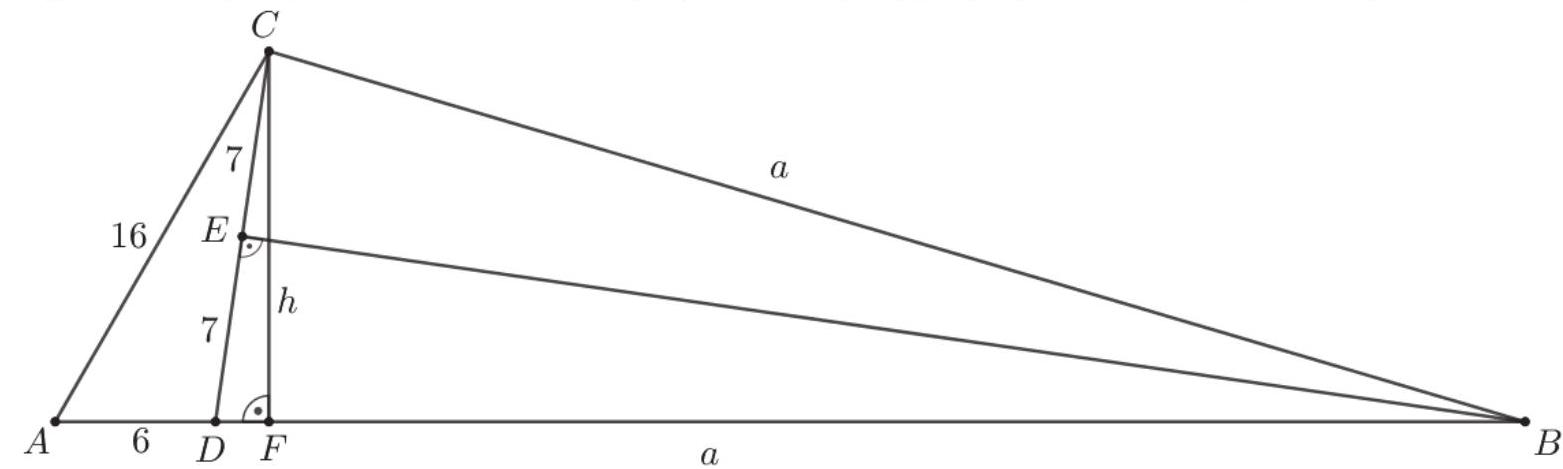
\includegraphics[max width=\textwidth, center]{2025_02_07_d712b9a47aa2c64928dbg-31}

Obliczmy pole trójkąta $A D C$ ze wzoru Herona.\\
Połowa obwodu tego trójkąta jest równa $p=\frac{16+14+6}{2}=18$, więc

$$
P_{A D C}=\sqrt{18 \cdot(18-16) \cdot(18-14) \cdot(18-6)}=\sqrt{18 \cdot 2 \cdot 4 \cdot 12}=24 \sqrt{3} .
$$

Odcinek $C F$ jest też wysokością trójkąta $A D C$, więc pole tego trójkąta jest równe

$$
P_{A D C}=\frac{1}{2} \cdot|A D| \cdot h=\frac{1}{2} \cdot 6 \cdot h=3 h .
$$

Otrzymujemy zatem

$$
\begin{aligned}
3 h & =24 \sqrt{3}, \\
h & =8 \sqrt{3} .
\end{aligned}
$$

Z twierdzenia Pitagorasa dla trójkąta $C D F$ otrzymujemy

$$
\begin{gathered}
|D F|^{2}=|C D|^{2}-|C F|^{2} \\
|D F|^{2}=14^{2}-(8 \sqrt{3})^{2}=4
\end{gathered}
$$

Stąd $|D F|=2$.\\
Trójkąt $B C D$ jest równoramienny, więc spodek $E$ wysokości $B E$ tego trójkąta jest środkiem podstawy $C D$. Zatem

$$
|D E|=\frac{1}{2} \cdot|C D|=\frac{1}{2} \cdot 14=7 .
$$

Trójkąty $C D F$ i $B D E$ są podobne, gdyż oba są prostokątne i mają wspólny kąt ostry przy wierzchołku $D$. Zatem

$$
\begin{gathered}
\frac{|D B|}{|D E|}=\frac{|C D|}{|D F|}, \\
\frac{a}{14}=\frac{7}{2}, \\
a=49 .
\end{gathered}
$$

Obwód trójkąta $A B C$ jest równy

$$
L_{A B C}=16+6+2 \cdot 49=120 .
$$

\section*{X sposób}
Przyjmijmy oznaczenia jak na rysunku.\\
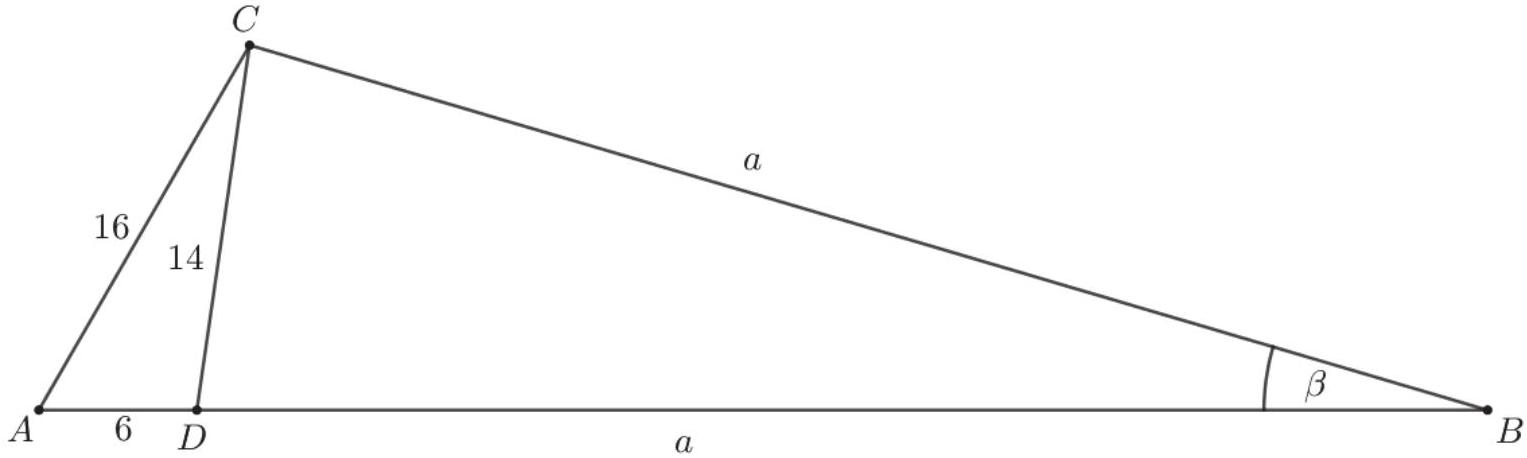
\includegraphics[max width=\textwidth, center]{2025_02_07_d712b9a47aa2c64928dbg-32}

Z twierdzenia cosinusów dla trójkąta $B C D$ otrzymujemy

$$
14^{2}=a^{2}+a^{2}-2 \cdot a \cdot a \cdot \cos \beta .
$$

Stąd

$$
\cos \beta=\frac{2 a^{2}-14^{2}}{2 a^{2}} .
$$

Z twierdzenia cosinusów dla trójkąta $A B C$ otrzymujemy

$$
16^{2}=(a+6)^{2}+a^{2}-2 \cdot(a+6) \cdot a \cdot \cos \beta .
$$

Stąd i z poprzednio otrzymanego równania otrzymujemy równanie z jedną niewiadomą $a$

$$
\begin{gathered}
16^{2}=(a+6)^{2}+a^{2}-2 \cdot(a+6) \cdot a \cdot \frac{2 a^{2}-14^{2}}{2 a^{2}}, \\
256 a=a(a+6)^{2}+a^{3}-(a+6)\left(2 a^{2}-196\right), \\
256 a=a^{3}+12 a^{2}+36 a+a^{3}-2 a^{3}-12 a^{2}+196 a+6 \cdot 196, \\
24 a=6 \cdot 196, \\
a=49 .
\end{gathered}
$$

Obwód trójkąta $A B C$ jest równy

$$
L_{A B C}=16+6+2 \cdot 49=120 .
$$

\section*{XI sposób}
Poprowadźmy wysokość $C F$ trójkąta $B C D$ i przyjmijmy oznaczenia jak na rysunku.\\
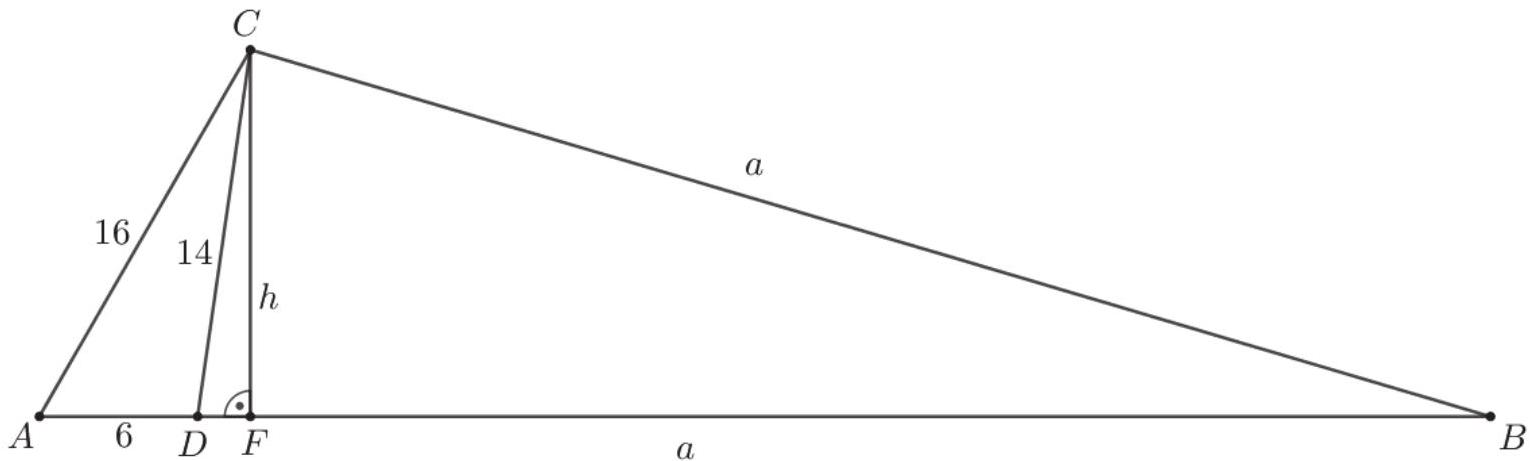
\includegraphics[max width=\textwidth, center]{2025_02_07_d712b9a47aa2c64928dbg-32(1)}

Obliczmy pole trójkąta $A D C$ ze wzoru Herona.\\
Połowa obwodu tego trójkąta jest równa $p=\frac{16+14+6}{2}=18$, więc

$$
P_{A D C}=\sqrt{18 \cdot(18-16) \cdot(18-14) \cdot(18-6)}=\sqrt{18 \cdot 2 \cdot 4 \cdot 12}=24 \sqrt{3} .
$$

Odcinek $C F$ jest też wysokością trójkąta $A D C$, więc pole tego trójkąta jest równe

$$
P_{A D C}=\frac{1}{2} \cdot|A D| \cdot h=\frac{1}{2} \cdot 6 \cdot h=3 h .
$$

Otrzymujemy zatem

$$
\begin{aligned}
3 h & =24 \sqrt{3}, \\
h & =8 \sqrt{3} .
\end{aligned}
$$

Pole trójkąta $B C D$ jest więc równe

$$
P_{B C D}=\frac{1}{2} \cdot|B D| \cdot h=\frac{1}{2} \cdot 8 \sqrt{3} \cdot a=4 \sqrt{3} \cdot a .
$$

Zapiszmy pole trójkąta $A B C$, stosując wzór Herona. Połowa obwodu trójkąta $A B C$ jest równa

$$
p=\frac{a+6+a+16}{2}=a+11,
$$

więc

$$
P_{A B C}=\sqrt{(a+11)(a+11-16)(a+11-a-6)(a+11-a)}=\sqrt{(a+11)(a-5) \cdot 5 \cdot 11} .
$$

Ponieważ $P_{A B C}=P_{A C D}+P_{B C D}$, więc otrzymujemy

$$
\sqrt{(a+11)(a-5) \cdot 5 \cdot 11}=24 \sqrt{3}+4 \sqrt{3} \cdot a .
$$

Obie strony tego równania są dodatnie, więc podnosząc je do kwadratu otrzymujemy równanie równoważne

$$
\begin{gathered}
(a+11)(a-5) \cdot 5 \cdot 11=1728+576 a+48 a^{2}, \\
55 a^{2}+330 a-3025=48 a^{2}+576 a+1728 . \\
7 a^{2}-246 a-4753=0 . \\
\Delta=(-246)^{2}-4 \cdot 7 \cdot(-4753)=193600, \sqrt{\Delta}=440, \\
a=\frac{246-440}{14}<0 \text { lub } a=\frac{246+440}{14}=49 .
\end{gathered}
$$

Obwód trójkąta $A B C$ jest równy

$$
L_{A B C}=16+6+2 \cdot 49=120 .
$$

\section*{Zadanie 11. (0-6)}
IV. Użycie i tworzenie strategii.\\
8. Geometria na płaszczyźnie kartezjańskiej. Zdający posługuje się równaniem okręgu $(x-a)^{2}+(y-b)^{2}=r^{2}$ oraz opisuje koła za pomocą nierówności (R8.5).

\section*{Schemat punktowania}
\section*{I. Rozwiązanie z wykorzystaniem odległości środków okręgów stycznych}
Rozwiązanie składa się z trzech etapów:\\
Pierwszy etap polega na wyznaczeniu środków i promieni obu podanych okręgów oraz ustaleniu warunków ogólnych ich położenia względem siebie.\\
Za poprawne rozwiązanie tego etapu zdający otrzymuje 2 punkty.\\
Drugi etap polega na wyznaczeniu równania z jedną niewiadomą, która opisuje warunek styczności zewnętrznej i rozwiązanie tego równania.\\
Za poprawne rozwiązanie tego etapu zdający otrzymuje 2 punkty.\\
Trzeci etap polega na wyznaczeniu równania z jedną niewiadomą, która opisuje warunek styczności wewnętrznej i rozwiązanie tego równania.\\
Za poprawne rozwiązanie tego etapu zdający otrzymuje 2 punkty.

\section*{Uwaga}
Etapy drugi i trzeci oceniane są niezależnie od siebie.\\
Podział punktów za pierwszy etap rozwiązania:\\
Zdający otrzymuje 2 punkty, gdy:\\
zapisze współrzędne środków i promienie obu okręgów:

$$
S_{1}=(6,4), r_{1}=3 \text { oraz } S_{2}=(a,-2), r_{2}=9
$$

oraz\\
zapisze warunki styczności obu okręgów w dwóch przypadkach:

$$
\left|S_{1} S_{2}\right|=r_{1}+r_{2}, \quad\left|S_{1} S_{2}\right|=r_{2}-r_{1} .
$$

Zdający otrzymuje 1 punkt, gdy:

\begin{itemize}
  \item zauważy i zapisze, że są dwa przypadki styczności okręgów, tj. styczność zewnętrzną i wewnętrzną\\
albo
  \item wyznaczy wspórrzędne środków okręgów i obliczy promienie obu okręgów.
\end{itemize}

Podział punktów za drugi etap rozwiązania:\\
Zdający otrzymuje 2 punkty, gdy zapisze równanie:

$$
\sqrt{(a-6)^{2}+6^{2}}=12
$$

i wyznaczy jego rozwiązania: $a=6(1+\sqrt{3})$ oraz $a=6(1-\sqrt{3})$.\\
Zdający otrzymuje 1 punkt, gdy zapisze równanie:

$$
\sqrt{(a-6)^{2}+6^{2}}=12 .
$$

\section*{Podział punktów za trzeci etap rozwiązania:}
Zdający otrzymuje 2 punkty, gdy zapisze równanie:

$$
\sqrt{(a-6)^{2}+6^{2}}=6
$$

i wyznaczy jego rozwiązanie: $a=6$.\\
Zdający otrzymuje 1 punkt, gdy zapisze równanie:

$$
\sqrt{(a-6)^{2}+6^{2}}=6 .
$$

\section*{Uwagi}
\begin{enumerate}
  \item Jeżeli zdający prowadzi poprawne rozumowanie na każdym etapie rozwiązania zadania i rozwiązuje zadanie do końca, ale popełnia jedynie błędy rachunkowe, to może otrzymać co najwyżej 5 punktów, o ile popełnione błędy nie ułatwiają rozważanego zagadnienia na żadnym etapie rozwiązania.
  \item Jeżeli zdający prowadzi poprawne rozumowanie na każdym etapie rozwiązania zadania, rozwiązuje zadanie do końca i jedynym błędem, który jednak nie ułatwia rozwiązania zadania na żadnym etapie rozwiązania, jest błąd, polegający na:\\
a) niepoprawnym wyznaczeniu promieni okręgów lub współrzędnych ich środków, to zdający otrzymuje co najwyżej 4 punkty;\\
b) zastosowaniu niepoprawnej metody wyznaczania odległości środków okręgów, to zdający otrzymuje co najwyżej 4 punkty;\\
c) zastosowaniu niepoprawnego wzoru „ $\sqrt{a^{2}+b^{2}}=\sqrt{a^{2}}+\sqrt{b^{2}}$ " lub , $(a \pm b)^{2}=a^{2} \pm b^{2}$ ", to zdający otrzymuje co najwyżej 4 punkty.
  \item Jeżeli zdający sporządzi poprawną ilustrację graficzną i na tej podstawie zapisze, że dla $a=6$ podane okręgi są styczne wewnętrznie i na tym zakończy, to otrzymuje 2 punkty.
  \item Jeżeli zdający rozważa tylko jeden przypadek styczności okręgów i w tym przypadku rozwiąże zadanie do końca, popełniając jeden błąd opisany w uwadze 2., to otrzymuje co najwyżej 2 punkty.
\end{enumerate}

\section*{II. Rozwiązanie z wykorzystaniem wspólnej stycznej lub równania kwadratowego z parametrem}
Zdający otrzymuje 6 punktów, gdy wyznaczy wszystkie wartości parametru $a$ : $a=6$ lub $a=6+6 \sqrt{3}$ lub $a=6-6 \sqrt{3}$.

Zdający otrzymuje 5 punktów, gdy wyznaczy tylko jedno z rozwiązań równania z jedną niewiadomą $a$ zapisze równanie kwadratowe z niewiadomą $a$, np.: $a=6$.

Zdający otrzymuje 4 punkty, gdy zapisze równanie wielomianowe z niewiadomą $a$ :

$$
\begin{gathered}
\left(a^{2}-12 a\right)^{2}=9\left(4 a^{2}-48 a+288\right) \text { lub } \\
4^{2}\left(a^{3}-6 a^{2}-72 a+864\right)^{2}-4 \cdot 4\left(a^{2}-12 a+72\right) \cdot\left(a^{4}-144 a^{2}+9072\right)=0 .
\end{gathered}
$$

Zdający otrzymuje $\mathbf{3}$ punkty, gdy

\begin{itemize}
  \item zapisze równanie z niewiadomą $a: \frac{\left|(12-2 a) \cdot 6+12 \cdot 4+a^{2}-120\right|}{\sqrt{(12-2 a)^{2}+12^{2}}}=3$\\
albo
  \item zapisze równanie kwadratowe z jedną niewiadomą $x$ (lub $y$ ) i parametrem $a$ oraz zapisze, że równanie to musi mieć jedno rozwiązanie, np.:
\end{itemize}

$$
x^{2}+\left(\left(1-\frac{1}{6} a\right) x+10-\frac{1}{12} a^{2}\right)^{2}-12 x-8\left(\left(1-\frac{1}{6} a\right) x+10-\frac{1}{12} a^{2}\right)+43=0 \text { oraz } \Delta=0 .
$$

Zdający otrzymuje 2 punkty, gdy

\begin{itemize}
  \item zapisze równanie prostej $(12-2 a) x+12 y+a^{2}-120=0$ oraz zapisze współrzędne środka i promień jednego z okręgów oraz zapisze, że okręgi mają dokładnie jeden punkt wspólny, gdy odległośc środka jednego okręgu od wspólnej stycznej tych okręgów jest równa promieniowi tego okręgu\\
albo
  \item zapisze równanie z jedną niewiadomą $x$ (lub $y$ ) i parametrem $a, \mathrm{np}$.:
\end{itemize}

$$
x^{2}+\left(\left(1-\frac{1}{6} a\right) x+10-\frac{1}{12} a^{2}\right)^{2}-12 x-8\left(\left(1-\frac{1}{6} a\right) x+10-\frac{1}{12} a^{2}\right)+43=0
$$

Zdający otrzymuje 1 punkt, gdy

\begin{itemize}
  \item zapisze równanie prostej $(12-2 a) x+12 y+a^{2}-120=0$\\
albo
  \item zapisze współrzędne środka i promień jednego z okręgów oraz zapisze, że okręgi mają dokładnie jeden punkt wspólny, gdy odległość środka jednego okręgu od wspólnej stycznej tych okręgów jest równa promieniowi tego okręgu.
\end{itemize}

\section*{Uwaga}
Jeżeli zdający zapisze równanie prostej, będącej osią potęgową okręgów i traktuje to równanie jak równanie kwadratowe zmiennej $a$, a następnie wyznacza konkretne wartości $x, y, a$, sprawdza dla wyznaczonych wartości prawdziwość równania osi potęgowej okręgów i podaje jedno $z$ rozwiązań zadania, to otrzymuje 3 punkty.

\section*{Przykładowe rozwiązania}
\section*{I sposób}
Okrąg o równaniu $x^{2}+y^{2}-12 x-8 y+43=0$ ma środek punkcie $S_{1}=(6,4)$ i promień $r_{1}=3$, a okrąg o równaniu $x^{2}+y^{2}-2 a x+4 y+a^{2}-77=0$ ma środek w punkcie $S_{2}=(a,-2)$ i promień $r_{2}=9$. Ponieważ te okręgi mają dokładnie jeden punkt wspólny, więc odległość pomiędzy środkami okręgów jest równa sumie promieni lub różnicy promieni:

$$
\left|S_{1} S_{2}\right|=r_{1}+r_{2} \text { lub }\left|S_{1} S_{2}\right|=r_{2}-r_{1}
$$

Otrzymujemy zatem równania

$$
\sqrt{(a-6)^{2}+6^{2}}=12 \text { lub } \sqrt{(a-6)^{2}+6^{2}}=6
$$

Zatem

$$
(a-6)^{2}=108 \text { lub }(a-6)^{2}=0
$$

Równanie $(a-6)^{2}=108$ ma dwa rozwiązania: $a=6(1+\sqrt{3})$ oraz $a=6(1-\sqrt{3})$, natomiast równanie $(a-6)^{2}=0$ ma jedno rozwiązanie $a=6$. Zatem podane okręgi są styczne zewnętrznie dla $a=6(1+\sqrt{3})$ lub dla $a=6(1-\sqrt{3})$, natomiast są okręgami stycznymi wewnętrznie dla $a=6$.

\section*{II sposób (wspólna styczna)}
Okrąg o równaniu $x^{2}+y^{2}-12 x-8 y+43=0$ ma środek $S_{1}=(6,4)$ i promień $r_{1}=3$, a okrąg o równaniu $x^{2}+y^{2}-2 a x+4 y+a^{2}-77=0$ ma środek $S_{2}=(a,-2)$ i promień $r_{2}=9$.\\
Okręgi te mają różne promienie, więc te okręgi mają dokładnie jeden punkt wspólny wtedy i tylko wtedy, gdy mają dokładnie jedną wspólną styczną. Tak jest wtedy i tylko wtedy, gdy odległość środka jednego z tych okręgów od tej stycznej jest równa promieniowi tego okręgu. Jeśli tę wspólną styczną oznaczymy przez $k$, to wtedy mamy

$$
\operatorname{odl}\left(S_{1}, k\right)=3 .
$$

Odejmując stronami równania okręgów otrzymujemy

$$
(12-2 a) x+12 y+a^{2}-120=0 .
$$

Jest to równanie wspólnej osi potęgowej tych okręgów. Jeśli teraz istnieją takie wartości parametru $a$, dla których spełniony jest warunek $\operatorname{odl}\left(S_{1}, k\right)=3$, to wtedy ta oś potęgowa jest jednocześnie wspólną styczną tych okręgów. Otrzymujemy zatem równanie

$$
\begin{aligned}
& \frac{\left|(12-2 a) \cdot 6+12 \cdot 4+a^{2}-120\right|}{\sqrt{(12-2 a)^{2}+12^{2}}}=3 \\
& \left|a^{2}-12 a\right|=3 \sqrt{4 a^{2}-48 a+288}
\end{aligned}
$$

Obie strony tego równania są nieujemne, więc podnosząc je do kwadratu otrzymujemy równanie równoważne

$$
\begin{gathered}
\left(a^{2}-12 a\right)^{2}=9\left(4 a^{2}-48 a+288\right), \\
a^{4}-24 a^{3}+144 a^{2}=36 a^{4}-432 a+2592, \\
a^{4}-24 a^{3}+108 a^{2}+432 a-2592=0, \\
a^{4}-12 a^{3}+36 a^{2}-12 a^{3}+144 a^{2}-432 a-72 a^{2}+864 a-2592=0, \\
a^{2}\left(a^{2}-12 a+36\right)-12 a\left(a^{2}-12 a+36\right)-72\left(a^{2}-12 a+36\right)=0, \\
\left(a^{2}-12 a-72\right)\left(a^{2}-12 a+36\right)=0, \\
\left(a^{2}-12 a+36-108\right)(a-6)^{2}=0, \\
\left((a-6)^{2}-36 \cdot 3\right)(a-6)^{2}=0, \\
(a-6-6 \sqrt{3})(a-6+6 \sqrt{3})(a-6)^{2}=0 .
\end{gathered}
$$

Stąd

$$
a=6+6 \sqrt{3} \text { lub } a=6-6 \sqrt{3} \text { lub } a=6 .
$$

III sposób (równanie kwadratowe z parametrem)\\
Okrąg o równaniu $x^{2}+y^{2}-12 x-8 y+43=0$ ma środek $S_{1}=(6,4)$ i promień $r_{1}=3$, a okrąg o równaniu $x^{2}+y^{2}-2 a x+4 y+a^{2}-77=0$ ma środek $S_{2}=(a,-2)$ i promień $r_{2}=9$.

Okręgi te mają różne promienie, więc te okręgi mają dokładnie jeden punkt wspólny wtedy i tylko wtedy, gdy układ równań

$$
x^{2}+y^{2}-12 x-8 y+43=0 \text { i } x^{2}+y^{2}-2 a x+4 y+a^{2}-77=0
$$

ma dokładnie jedno rozwiązanie. Stąd otrzymujemy kolejno

$$
\begin{gathered}
(12-2 a) x+12 y+a^{2}-120=0 \text { i } x^{2}+y^{2}-12 x-8 y+43=0 \\
y=\left(1-\frac{1}{6} a\right) x+10-\frac{1}{12} a^{2} \text { i } x^{2}+y^{2}-12 x-8 y+43=0 .
\end{gathered}
$$

Stąd otrzymujemy równanie z niewiadomą $x$ i parametrem $a$

$$
\begin{aligned}
& x^{2}+\left(\left(1-\frac{1}{6} a\right) x+10-\frac{1}{12} a^{2}\right)^{2}-12 x-8\left(\left(1-\frac{1}{6} a\right) x+10-\frac{1}{12} a^{2}\right)+43=0, \\
& 4\left(a^{2}-12 a+72\right) x^{2}-4\left(a^{3}-6 a^{2}-72 a+864\right) x+a^{4}-144 a^{2}+9072=0
\end{aligned}
$$

Ponieważ $a^{2}-12 a+72=(a-6)^{2}+36>0$ dla każdego $a$, więc równanie jest kwadratowe. Zatem układ równań ma dokładnie jedno rozwiązanie wtedy i tylko wtedy, gdy to równanie ma dokładnie jedno rozwiązanie, a tak jest wtedy i tylko wtedy, gdy wyróżnik trójmianu kwadratowego $\quad 4\left(a^{2}-12 a+72\right) x^{2}-4\left(a^{3}-6 a^{2}-72 a+864\right) x+a^{4}-144 a^{2}+9072$ jest równy 0 . Otrzymujemy więc równanie

$$
\begin{gathered}
4^{2}\left(a^{3}-6 a^{2}-72 a+864\right)^{2}-4 \cdot 4\left(a^{2}-12 a+72\right) \cdot\left(a^{4}-144 a^{2}+9072\right)=0, \\
\left(a^{3}-6 a^{2}-72 a+864\right)^{2}-\left(a^{2}-12 a+72\right) \cdot\left(a^{4}-144 a^{2}+9072\right)=0, \\
-36 a^{4}+864 a^{3}-3888 a^{2}-15552 a+93312=0, \\
-36 a^{4}+864 a^{3}-3888 a^{2}-15552 a+93312=0, \\
a^{4}-24 a^{3}+108 a^{2}+432 a-2592=0, \\
a^{4}-12 a^{3}+36 a^{2}-12 a^{3}+144 a^{2}-432 a-72 a^{2}+864 a-2592=0, \\
a^{2}\left(a^{2}-12 a+36\right)-12 a\left(a^{2}-12 a+36\right)-72\left(a^{2}-12 a+36\right)=0, \\
\left(a^{2}-12 a-72\right)\left(a^{2}-12 a+36\right)=0, \\
\left(a^{2}-12 a+36-108\right)(a-6)^{2}=0, \\
\left((a-6)^{2}-36 \cdot 3\right)(a-6)^{2}=0, \\
(a-6-6 \sqrt{3})(a-6+6 \sqrt{3})(a-6)^{2}=0 .
\end{gathered}
$$

Stąd

$$
a=6+6 \sqrt{3} \text { lub } a=6-6 \sqrt{3} \text { lub } a=6 .
$$

Zadanie 12. (0-6)\\
IV. Użycie i tworzenie strategii.\\
5. Ciągi. Zdający stosuje wzór na $n$-ty wyraz i na sumę $n$ początkowych wyrazów ciągu arytmetycznego (5.3). Zdający stosuje wzór na $n$-ty wyraz i na sumę $n$ początkowych wyrazów ciągu geometrycznego (5.4).

\section*{Schemat punktowania}
Rozwiązanie składa się z dwóch etapów:\\
Pierwszy etap polega na wyznaczeniu zależności niezbędnych do obliczenia $q$.\\
Za poprawne rozwiązanie tego etapu zdający otrzymuje 4 punkty.\\
Drugi etap polega na wyznaczeniu wartości ilorazu ciągu geometrycznego.\\
Za poprawne rozwiązanie tego etapu zdający otrzymuje 2 punkty.

\section*{Uwaga}
Zdający może rozpocząć realizację drugiego etapu przed podjęciem działań koniecznych do realizacji pierwszego etapu.

Podział punktów za pierwszy etap rozwiązania:\\
Zdający otrzymuje 4 punkty, gdy:

\begin{itemize}
  \item zapisze poprawne zależności między wyrazami ciągu:
\end{itemize}

$$
\begin{aligned}
& a=\frac{1}{3} c, b=\frac{2}{3} c \quad \text { albo } \quad c=3 a, b=2 a, \\
& \text { albo } \quad \frac{a}{b}=\frac{1}{2} \quad \text { albo } \quad \frac{r}{a}=1 .
\end{aligned}
$$

albo

\begin{itemize}
  \item zapisze równanie kwadratowe z niewiadomą $q$ :
\end{itemize}

$$
3 q^{2}+8 q-3=0
$$

Zdający otrzymuje 3 punkty, gdy:

\begin{itemize}
  \item rozwiąże równanie z niewiadomymi $a \mathrm{i} c$ :
\end{itemize}

$$
a_{1}=-\frac{9}{13} c \quad \text { lub } \quad a_{2}=\frac{1}{3} c \quad \text { albo } \quad c_{1}=-\frac{13}{9} a \quad \text { lub } \quad c_{2}=3 a
$$

albo

\begin{itemize}
  \item zapisze równanie kwadratowe z niewiadoma $\frac{a}{b}$ lub $\frac{r}{a}$ :
\end{itemize}

$$
\left(\frac{a}{b}\right)^{2}+4 \frac{a}{b}-\frac{9}{4}=0 \text { lub } 9\left(\frac{r}{a}\right)^{2}+2 \frac{r}{a}-11=0 .
$$

Zdający otrzymuje 2 punkty, gdy zapisze równanie z dwiema niewiadomymi:

\begin{itemize}
  \item np.: $a \mathrm{i} c, \frac{9}{4}\left(\frac{a+c}{2}\right)^{2}=2 a^{2}+2 a \cdot\left(\frac{a+c}{2}\right)+a c$\\
albo
  \item np.: $a \mathrm{i} r, \frac{4}{9 a^{2}+18 a r+9 r^{2}}=\frac{1}{5 a^{2}+4 a r}$.
\end{itemize}

Zdający otrzymuje 1 punkt, gdy\\
zapisze zależności wynikające $z$ zastosowania własności ciągów arytmetycznego i geometrycznego,\\
np.: $b=\frac{a+c}{2},\left(\frac{2}{3 b}\right)^{2}=\frac{1}{a} \cdot \frac{1}{2 a+2 b+c}$ lub $b=a+r, c=a+2 r,\left(\frac{2}{3 b}\right)^{2}=\frac{1}{a} \cdot \frac{1}{2 a+2 b+c}$.

Podział punktów za drugi etap rozwiązania:\\
Zdający otrzymuje 2 punkty, gdy obliczy wartość ilorazu ciągu geometrycznego: $q=\frac{1}{3}$.\\
Zdający otrzymuje 1 punkt, gdy wyrazi iloraz ciągu geometrycznego jako funkcję dwóch zmiennych, np.: $q=\frac{\frac{2}{3 b}}{\frac{1}{a}}=\frac{2 a}{3 b}$ lub $q=\frac{2}{3} \cdot \frac{a}{a+r}$.

\section*{Uwagi}
\begin{enumerate}
  \item Jeżeli zdający realizuje strategię rozwiązania i popełnia jedynie błędy rachunkowe, to może otrzymać 5 punktów, o ile popełnione błędy nie ułatwiają rozważanego zagadnienia na żadnym etapie rozwiązania.
  \item Jeżeli zdający realizuje strategię rozwiązania i jedynym błędem, który jednak nie ułatwia rozważania zagadnienia na żadnym etapie rozwiązania, jest błąd, polegający na niepoprawnym zastosowaniu własności ciągu arytmetycznego albo ciągu geometrycznego, to zdający otrzymuje co najwyżej 4 punkty.
  \item Jeżeli zdający pomyli ciąg arytmetyczny z geometrycznym, to za całe rozwiązanie otrzymuje $\mathbf{0}$ punktów, o ile nie uzyska punktu za wyznaczenie $q$ w zależności od dwóch zmiennych, np.: $q=\frac{\frac{2}{3 b}}{\frac{1}{a}}=\frac{2 a}{3 b}$.
  \item Jeżeli zdający nie otrzyma równania kwadratowego zupełnego z dwiema niewiadomymi, to uznajemy, że znacznie ułatwił sobie rozwiązanie i za pierwszy etap rozwiązania może otrzymać co najwyżej 2 punkty.
  \item Jeżeli zdający wyznacza $q$ jedynie na podstawie konkretnych wartości wyrazów ciągów arytmetycznego i geometrycznego, to otrzymuje co najwyżej 1 punkt.
\end{enumerate}

\section*{Przykładowe rozwiązanie}
Zakładamy, że $a \neq 0, b \neq 0, a+b+c \neq 0$.\\
Ciąg $(a, b, c)$ jest ciągiem arytmetycznym, a zatem:

$$
b=\frac{a+c}{2} .
$$

$\operatorname{Ciaqg}\left(\frac{1}{a}, \frac{2}{3 b}, \frac{1}{2 a+2 b+c}\right)$ jest ciągiem geometrycznym, a zatem:

$$
\left(\frac{2}{3 b}\right)^{2}=\frac{1}{a} \cdot \frac{1}{2 a+2 b+c}
$$

stąd po przekształceniach otrzymujemy:

$$
\frac{9}{4} b^{2}=a(2 a+2 b+c) .
$$

Po podstawieniu $b$ otrzymujemy:

$$
\begin{aligned}
& \frac{9}{4}\left(\frac{a+c}{2}\right)^{2}=2 a^{2}+2 a \cdot\left(\frac{a+c}{2}\right)+a c \\
& \frac{9}{4} \cdot \frac{a^{2}+2 a c+c^{2}}{4}=2 a^{2}+2 \frac{a^{2}+a c}{2}+a c \\
& 9\left(a^{2}+2 a c+c^{2}\right)=32 a^{2}+16 a^{2}+16 a c+16 a c
\end{aligned}
$$

Równanie można doprowadzić do postaci:

$$
-39 a^{2}-14 a c+9 c^{2}=0 \quad \text { lub } \quad 9 c^{2}-14 a c-39 a^{2}=0
$$

Wyróżnik trójmianu kwadratowego $-39 a^{2}-14 a c+9 c^{2}(a$ traktujemy jako zmienną) jest równy

$$
\Delta=1600 c^{2}, \quad \sqrt{\Delta}=40 c .
$$

Wyróżnik trójmianu kwadratowego $9 c^{2}-14 a c-39 a^{2}$ ( $c$ traktujemy jako zmienną) jest równy

$$
\Delta=1600 a^{2}, \quad \sqrt{\Delta}=40 a .
$$

Stąd pierwiastki równań odpowiednio $-39 a^{2}-14 a c+9 c^{2}=0$ i $9 c^{2}-14 a c-39 a^{2}=0$ są równe:

$$
a_{1}=-\frac{9}{13} c \quad \text { lub } \quad a_{2}=\frac{1}{3} c \quad \text { oraz } \quad c_{1}=-\frac{13}{9} a \text { lub } c_{2}=3 a .
$$

Rozwiązania $a_{1}=-\frac{9}{13} c$ i $c_{1}=-\frac{13}{9} a$ są sprzeczne z założeniem o dodatniości wyrazów ciągu arytmetycznego.

A zatem $b=\frac{2}{3} c$ lub $b=2 a$.

Iloraz ciągu geometrycznego jest równy $q=\frac{\frac{2}{3 b}}{\frac{1}{a}}=\frac{2 a}{3 b}$, a zatem $q=\frac{1}{3}$.\\
Odp.: Iloraz ciągu geometrycznego $q=\frac{1}{3}$.

\section*{Uwaga}
Możemy też w rozwiązaniu zauważyć, że $q=\frac{2}{3} \cdot \frac{a}{b}$ i $c=2 b-a$.

Wówczas otrzymamy równanie kwadratowe: $3 q^{2}+8 q-3=0$.\\
Wyznaczamy dwa rozwiązania tego równania: $q=-3$ lub $q=\frac{1}{3}$.\\
Zauważamy, że tylko $q=\frac{1}{3}$ spełnia warunki zadania.

\section*{Zadanie 13. (0-6)}
IV. Użycie i tworzenie strategii.\\
3. Równania i nierówności. Zdający stosuje twierdzenie o reszcie z dzielenia wielomianu przez dwumian $x-a$ (R3.4). Zdający rozwiązuje łatwe nierówności wielomianowe (R3.7).

\section*{Schemat punktowania}
Rozwiązanie składa się z dwóch etapów:\\
Pierwszy etap polega na wyznaczeniu wartości parametru $m$, dla której spełnione są warunki określone w zadaniu. Za poprawne rozwiązanie tego etapu zdający otrzymuje 4 punkty, przy czym otrzymuje:\\
4 punkty, gdy uzasadni, że jedyną wartością parametru $m$ jest $m=1$,\\
3 punkty, gdy

\begin{itemize}
  \item zapisze oba równania wynikające z treści zadania, np.:
\end{itemize}

$$
\begin{aligned}
& 2 \cdot 2^{3}+\left(m^{3}+2\right) \cdot 2^{2}-11 \cdot 2-2(2 m+1)=0 \\
& 2 \cdot(-1)^{3}+\left(m^{3}+2\right) \cdot(-1)^{2}-11 \cdot(-1)-2(2 m+1)=6
\end{aligned}
$$

i rozwiąże przynajmniej jedno z nich\\
lub

\begin{itemize}
  \item rozwiąże równanie wynikające z tego układu, np.: $4 m^{3}-4 m=m^{3}-4 m+3$,
\end{itemize}

2 punkty, gdy

\begin{itemize}
  \item zapisze oba równania wynikające z treści zadania, np.:
\end{itemize}

$$
\begin{aligned}
& 2 \cdot 2^{3}+\left(m^{3}+2\right) \cdot 2^{2}-11 \cdot 2-2(2 m+1)=0 \\
& 2 \cdot(-1)^{3}+\left(m^{3}+2\right) \cdot(-1)^{2}-11 \cdot(-1)-2(2 m+1)=6
\end{aligned}
$$

albo

\begin{itemize}
  \item zapisze tylko jedno równanie wynikające $z$ treści zadania i rozwiąże je np.:
\end{itemize}

$$
2 \cdot 2^{3}+\left(m^{3}+2\right) \cdot 2^{2}-11 \cdot 2-2(2 m+1)=0, \text { skąd } m=0, m=-1, m=1
$$

1 punkt, gdy zapisze jedno z równań wynikających z treści zadania, np.: $2 \cdot 2^{3}+\left(m^{3}+2\right) \cdot 2^{2}-11 \cdot 2-2(2 m+1)=0,2 \cdot(-1)^{3}+\left(m^{3}+2\right) \cdot(-1)^{2}-11 \cdot(-1)-2(2 m+1)=6$.

Drugi etap polega na rozwiązaniu nierówności wielomianowej.\\
Za poprawne rozwiązanie tego etapu zdający otrzymuje 2 punkty, przy czym zdający otrzymuje 2 punkty gdy rozwiąże nierówność: $x \in(-\infty,-3\rangle \cup\left\langle-\frac{1}{2}, 2\right\rangle$.\\
Zdający otrzymuje 1 punkt gdy wyznaczy wszystkie pierwiastki wielomianu $2 x^{3}+3 x^{2}-11 x-6: x_{1}=-3, x_{2}=-\frac{1}{2}, x_{3}=2$.

\section*{Uwagi}
\begin{enumerate}
  \item Jeżeli zdający po zapisaniu układu równań jedynie zapisze $m=1$, to otrzymuje $\mathbf{3}$ punkty za pierwszy etap rozwiązania, jeśli natomiast opatrzy to odpowiednim komentarzem, np.: ,,jedynym rozwiązaniem układu równań jest $m=1$ ", to otrzymuje 4 punkty.
  \item Jeżeli zdający poprawnie interpretuje treść zadania $W(2)=0$ i $W(-1)=6$, ale popełnia błędy rachunkowe, zapisując równania wynikające z tych warunków, to za I etap może otrzymać co najwyżej $\mathbf{3}$ punkty, o ile popełnione błędy nie ułatwiają rozwiązania układu i układ nie jest sprzeczny.
  \item Jeżeli zdający popełnia błędy w interpretacji treści zadania, zapisując np. $W(-2)=0$ i $W(1)=6$, w konsekwencji których zapisuje błędne równania wynikające z tych warunków, to za I etap otrzymuje $\mathbf{0}$ punktów.
  \item Jeżeli zdający w wyniku błędów otrzyma wielomian $W(x)$, który ma trzy różne pierwiastki, przy czy jednym z nich jest liczba 2, to może otrzymać 2 punkty za drugi etap, o ile konsekwentnie rozwiąże otrzymaną nierówność.
  \item Jeżeli zdający w wyniku błędów rachunkowych otrzyma wielomian $W(x)$, który ma trzy różne pierwiastki, przy żadnym z nich nie jest liczba 2 , to zdający może otrzymać $\mathbf{1}$ punkt za drugi etap, o ile konsekwentnie rozwiąże otrzymaną nierówność.
  \item Jeżeli zdający w wyniku błędów rachunkowych otrzyma wielomian $W(x)$, który ma co najwyżej dwa pierwiastki (nie liczymy krotności pierwiastków), to otrzymuje $\mathbf{0}$ punktów za drugi etap.
  \item Przy rozwiązaniu układu równań wynikającego z treści zadania metodą opisaną w III sposobie, jak poniżej, akceptujemy sytuację, w której zdający nie zapisze, że liczba $m=1$ spełnia oba równania układu.
  \item Jeżeli zdający w I etapie rozwiązania obiera III sposób, opisany poniżej, i popełnia jedynie błąd rachunkowy przy rozwiązywaniu układu równań, ale otrzymuje jedną wartość m , to może otrzymać co najwyżej 5 punktów za całe rozwiązanie, o ile konsekwentnie rozwiąże zadanie do końca.
\end{enumerate}

\section*{Przykładowe rozwiązanie}
Rozwiązanie składa się z dwóch etapów.

\section*{Pierwszy etap}
Wielomian $W(x)$ jest podzielny przez dwumian $x-2$, więc 2 jest pierwiastkiem tego wielomianu. Zatem $W(2)=0$. Stąd otrzymujemy

$$
\begin{gathered}
16+4 m^{3}+8-22-4 m-2=0, \\
4 m^{3}-4 m=0 .
\end{gathered}
$$

Przy dzieleniu wielomianu $W(x)$ przez dwumian $x+1$ otrzymujemy resztę 6 , więc $W(-1)=6$. Stąd otrzymujemy

$$
\begin{gathered}
-2+m^{3}+2+11-4 m-2=6, \\
m^{3}-4 m+3=0 .
\end{gathered}
$$

Rozwiązujemy układ równań $\left\{\begin{array}{l}4 m^{3}-4 m=0 \\ m^{3}-4 m+3=0 .\end{array}\right.$

\section*{I sposób}
Z równania $4 m^{3}-4 m=0$ otrzymujemy rozwiązania: $m=0, m=-1, m=1$.\\
$Z$ tych trzech liczb tylko liczba 1 spełnia drugie równanie, zatem liczba 1 jest rozwiązaniem układu równań.

\section*{II sposób}
Z równania $m^{3}-4 m+3=0$ otrzymujemy rozwiązania: $m=1, \quad m=\frac{-1-\sqrt{13}}{2}, \quad m=\frac{-1+\sqrt{13}}{2}$. Z tych trzech liczb tylko liczba 1 spełnia pierwsze równanie, zatem liczba 1 jest rozwiązaniem układu równań.

\section*{III sposób}
Przyrównując lewe strony obu równań $\left\{\begin{array}{l}4 m^{3}-4 m=0 \\ m^{3}-4 m+3=0\end{array}\right.$ otrzymujemy

$$
\begin{aligned}
& \left\{\begin{array}{l}
4 m^{3}-4 m=m^{3}-4 m+3 \\
4 m^{3}-4 m=0
\end{array}\right. \\
& \left\{\begin{array}{l}
3 m^{3}-3=0 \\
4 m^{3}-4 m=0
\end{array}\right. \\
& \left\{\begin{array} { l } 
{ m ^ { 3 } = 1 } \\
{ 4 m ^ { 3 } - 4 m = 0 }
\end{array} \text { i } \left\{\begin{array}{l}
m=1 \\
4 m^{3}-4 m=0
\end{array}\right.\right.
\end{aligned}
$$

Sprawdzamy, czy liczba 1 spełnia jedno z równań:\\
$4 m^{3}-4 m=0$\\
$4 \cdot 1^{3}-4 \cdot 1=4-4=0$\\
lub\\
$m^{3}-4 m+3=0$\\
$1^{3}-4 \cdot 1+3=4-4=0$\\
Liczba $m=1$ spełnia każde z równań układu, więc jest jedynym rozwiązaniem tego układu.

\section*{Drugi etap}
Dla $m=1$ nierówność $W(x) \leq 0$ przyjmuje postać

$$
2 x^{3}+3 x^{2}-11 x-6 \leq 0
$$

Rozwiązujemy tę nierówność stosując przekształcenia równoważne i otrzymujemy kolejno:

$$
\begin{aligned}
& (x-2)\left(2 x^{2}+7 x+3\right) \leq 0 \\
& 2(x-2)(x+3)\left(x+\frac{1}{2}\right) \leq 0
\end{aligned}
$$

Zbiorem rozwiązań nierówności jest $(-\infty,-3\rangle \cup\left\langle-\frac{1}{2}, 2\right\rangle$.

\section*{Zadanie 14. (0-4)}
IV. Użycie i tworzenie strategii.\\
6. Trygonometria. Zdający stosuje wzory na sinus i cosinus sumy i różnicy kątów, sumę i różnicę sinusów i cosinusów kątów (R6.5).

\section*{Schemat punktowania}
Rozwiązanie petne 4 p.

Zdający zapisze rozwiązanie:

\begin{itemize}
  \item $x=k \pi \quad$ lub $\quad x=\frac{\pi}{3}+2 k \pi$, lub $\quad x=-\frac{\pi}{3}+2 k \pi$,\\
albo
  \item $x=\frac{\pi}{3}+\frac{2}{3} k \pi$ lub $x=2 k \pi$,\\
gdzie $k$ jest liczbą całkowitą.\\
Pokonanie zasadniczych trudności zadania
\end{itemize}

\section*{Zdający}
\begin{itemize}
  \item rozwiąże jedno z równań otrzymanej alternatywy:
  \item $\sin x=0: \quad x=k \pi$ lub $\cos x-\frac{1}{2}=0: \quad x=\frac{\pi}{3}+2 k \pi$ lub $x=-\frac{\pi}{3}+2 k \pi$, gdzie $k$ jest liczbą całkowitą, albo
  \item $\cos \frac{3 x}{2}=0: x=\frac{\pi}{3}+\frac{2}{3} k \pi$ lub $\sin \frac{x}{2}=0: x=2 k \pi$, gdzie $k$ jest liczbą całkowita,\\
albo
  \item wykorzysta równość $\sin 2 x=\sin x$ i zapisze: $2 x=x+2 k \pi$ lub $2 x=\pi-x+2 k \pi$, gdzie $k$ jest liczbą całkowitą.\\
i na tym zakończy lub dalej popełni błędy.\\
Rozwiązanie, w którym jest istotny postęp 2 p.
\end{itemize}

\section*{Zdający}
\begin{itemize}
  \item przekształci równanie równoważnie do alternatywy dwóch równań, np.: $\sin x=0 \quad$ lub $\quad \cos x-\frac{1}{2}=0, \cos \frac{3 x}{2}=0 \quad$ lub $\quad \sin \frac{x}{2}=0$\\
albo
  \item zapisze równanie w postaci $\sin 2 x=\sin x$ i zapisze jedną z prawdziwych zależności między kątami, których sinusy są równe, np. $2 x=x+2 k \pi$ lub $2 x=\pi-x+2 k \pi$,\\
albo
  \item zapisze jedno z równań $\sin x=0$ lub $\cos x-\frac{1}{2}=0$, lub $\cos \frac{3 x}{2}=0$, lub $\quad \sin \frac{x}{2}=0$ i rozwiąże je poprawnie do końca\\
i na tym zakończy lub dalej popełni błędy.
\end{itemize}

\section*{Rozwiązanie, w którym postęp jest niewielki, ale konieczny na drodze do pełnego rozwiązania zadania}
Zdający przekształci równanie równoważnie do postaci, w której występują funkcje sin i cos kąta $x$, np.: $\cos x\left[2 \sin x \cdot \cos \frac{\pi}{3}\right]=\frac{1}{2} \sin x$\\
i na tym zakończy lub dalej popełni błędy.

\section*{Uwagi}
\begin{enumerate}
  \item Jeżeli zdający przed uzyskaniem elementarnych równań trygonometrycznych popełnia jeden błąd, polegający na niepoprawnym zastosowaniu wzoru: na sumę sinusów lub na sinus sumy lub na sinus różnicy lub na sinus kąta podwojonego albo dzieli obie strony równania przez $\sin x$ i nie rozważa przypadku $\sin x=0$, to może otrzymać co najwyżej 2 punkty za całe rozwiązanie, o ile w rezultacie konsekwentnego postępowania otrzyma w wyniku końcowym przynajmniej dwie serie rozwiązań.
  \item Jeżeli zdający przed uzyskaniem elementarnych równań trygonometrycznych błędnie podstawia wartość funkcji trygonometrycznej konkretnego kąta, to może otrzymać co najwyżej 2 punkty za całe rozwiązanie.
  \item Jeżeli przy zapisie serii rozwiązań zdający błędnie zapisze część $z$ wielokrotnością kąta $\pi$, to otrzymuje co najwyżej $\mathbf{3}$ punkty za całe rozwiązanie.
  \item Jeżeli zdający przy zapisie rozwiązań obu równań pominie część z wielokrotnością kąta $\pi$, to otrzymuje 3 punkty za całe rozwiązanie, o ile zapisze wszystkie rozwiązania z przedziału domkniętego długości $2 \pi$.
  \item Jeżeli zdający popełnia błąd merytoryczny, polegający na:
\end{enumerate}

\begin{itemize}
  \item podniesieniu obu stron równania do potęgi drugiej bez sprawdzenia czy otrzymane w efekcie dalszego rozumowania wyniki spełniają równanie\\
lub
  \item podstawieniu w miejsce $\cos x$ wyrażenia $\sqrt{1-\sin ^{2} x}$,\\
to może otrzymać co najwyżej 2 punkty za całe rozwiązanie, o ile w rezultacie konsekwentnego postępowania otrzyma w wyniku końcowym przynajmniej dwie serie rozwiązań.
\end{itemize}

\begin{enumerate}
  \setcounter{enumi}{5}
  \item Jeżeli zdający przed uzyskaniem elementarnych równań trygonometrycznych popełnia co najmniej dwa błędy opisane w uwadze 1 . to może otrzymać co najwyżej 1 punkt za całe rozwiązanie, przy czym może go otrzymać tylko za pierwszy krok rozwiązania, tj. za przekształcenie równania do postaci równania z niewiadomymi $\sin x$ oraz $\cos x$.
\end{enumerate}

\section*{Przykładowe rozwiązania}
I sposób\\
Przekształcamy równanie i otrzymujemy:

$$
\begin{gathered}
\cos x\left[2 \sin x \cdot \cos \frac{\pi}{3}\right]=\frac{1}{2} \sin x \\
\sin x \cdot \cos x-\frac{1}{2} \sin x=0 \\
\sin x \cdot\left(\cos x-\frac{1}{2}\right)=0 \\
\sin x=0 \quad \text { lub } \quad \cos x-\frac{1}{2}=0
\end{gathered}
$$

Rozwiązania to:

$$
x=k \pi \quad \text { lub } \quad x=\frac{\pi}{3}+2 k \pi, \quad \operatorname{lub} x=-\frac{\pi}{3}+2 k \pi,
$$

gdzie $k$ jest liczbą całkowitą.\\
II sposób\\
Przekształcamy równanie i otrzymujemy:

$$
\begin{gathered}
\cos x\left[2 \sin x \cdot \cos \frac{\pi}{3}\right]=\frac{1}{2} \sin x \\
\sin x \cdot \cos x-\frac{1}{2} \sin x=0 \\
2 \sin x \cdot \cos x-\sin x=0 \\
\sin 2 x-\sin x=0 \\
2 \cos \frac{3 x}{2} \cdot \sin \frac{x}{2}=0 \\
\cos \frac{3 x}{2}=0 \quad \text { lub } \quad \sin \frac{x}{2}=0 \\
\frac{3 x}{2}=\frac{\pi}{2}+k \pi \quad \text { lub } \quad \frac{x}{2}=k \pi
\end{gathered}
$$

$$
x=\frac{\pi}{3}+\frac{2}{3} k \pi \quad \text { lub } \quad x=2 k \pi, \text { gdzie } k-\text { liczba całkowita. }
$$

III sposób\\
Przekształcamy równanie i otrzymujemy:

$$
\begin{gathered}
\cos x\left[2 \sin x \cdot \cos \frac{\pi}{3}\right]=\frac{1}{2} \sin x, \\
\sin x \cdot \cos x-\frac{1}{2} \sin x=0, \\
2 \sin x \cdot \cos x-\sin x=0, \\
\sin 2 x-\sin x=0, \\
\sin 2 x=\sin x, \\
2 x=x+2 k \pi \quad \text { lub } \quad 2 x=\pi-x+2 k \pi, \\
x=2 k \pi \quad \text { lub } \quad x=\frac{\pi}{3}+\frac{2}{3} k \pi, \text { gdzie } k-\text { liczba całkowita. }
\end{gathered}
$$

Zadanie 15. (0-7)

\begin{center}
\begin{tabular}{|l|l|}
\hline
\begin{tabular}{l}
III. Modelowanie \\
matematyczne. \\
\end{tabular} & \begin{tabular}{l}
11. Rachunek różniczkowy. Zdający stosuje pochodne do \\
rozwiązywania zagadnień optymalizacyjnych. \\
\end{tabular} \\
\hline
\end{tabular}
\end{center}

\section*{Schemat punktowania}
Rozwiązanie składa się z trzech etapów.\\
Pierwszy etap składa się z trzech części:

\begin{itemize}
  \item oznaczenia krawędzi podstawy i wysokości graniastosłupa, np. odpowiednio przez $a$ i $h$, oraz wyznaczenia wysokości graniastosłupa $h$ w zależności od zmiennej $a$ :
\end{itemize}

$$
h=\frac{8}{a^{2} \sqrt{3}} .
$$

\begin{itemize}
  \item zapisania pola powierzchni całkowitej graniastosłupa jako funkcji jednej zmiennej:\\
$f(a)=\frac{a^{2} \sqrt{3}}{2}+\frac{8 \sqrt{3}}{a}=\frac{a^{3} \sqrt{3}+16 \sqrt{3}}{2 a}$.
  \item wyznaczenia dziedziny funkcji $f:(0 ;+\infty)$.
\end{itemize}

Za poprawne rozwiązanie tego etapu zdający otrzymuje $\mathbf{3}$ punkty.

\section*{Uwagi do etapu I}
I. 1. Za drugą część tego etapu zdający może otrzymać punkt w dwóch przypadkach:

\begin{itemize}
  \item pierwszą część wykona bezbłędnie\\
albo
  \item błędnie wyznaczy $h$ w zależności od $a$, ale otrzyma wartość $h=k \cdot a^{-2}$, gdzie $k$ jest liczbą niewymierną.\\
I. 2. Punkt za część trzecią (wyznaczenie dziedziny funkcji) zdający otrzymuje niezależnie od realizacji dwóch pierwszych części tego etapu, pod warunkiem, że rozważa wyznaczoną przez siebie funkcję jednej zmiennej.
\end{itemize}

Drugi etap składa się z trzech części:

\begin{itemize}
  \item wyznaczenia wzoru pochodnej funkcji $f: f^{\prime}(a)=\frac{4 a^{3} \sqrt{3}-32 \sqrt{3}}{4 a^{2}}$.
  \item obliczenia miejsca zerowego pochodnej funkcji $f: a=2$.
  \item zbadania znaku pochodnej funkcji $f: f^{\prime}(a)>0$ dla $a \in(2 ;+\infty), f^{\prime}(a)<0$ dla $a \in(0 ; 2)$ i uzasadnienia, że dla $a=2$ funkcja $f$ osiąga wartość najmniejszą.
\end{itemize}

Za poprawne rozwiązanie tego etapu zdający otrzymuje $\mathbf{3}$ punkty.

\section*{Uwagi do etapu II}
II. 1. Jeżeli zdający wyznaczy pochodną funkcji z błędem, ale wyznaczona pochodna ma postać: $A a+\frac{B}{a^{2}}$, gdzie $A, B$ są liczbami niewymiernymi, lub postać ułamka, w którego liczniku jest wielomian stopnia trzeciego, a w mianowniku $m a^{2}$, to zdający może otrzymać punkty za część 2. i 3. tego etapu, o ile konsekwentnie obliczy miejsca zerowe pochodnej lub uzasadni istnienie najmniejszej wartości rozważanej funkcji.\\
II. 2. Badanie znaku pochodnej zdający może opisać w inny sposób, np. szkicując wykres funkcji, która w ten sam sposób jak pochodna zmienia znak.\\
II. 3. Za poprawne uzasadnienie, że rozważana funkcja posiada wartość najmniejszą dla wyznaczonej wartości $a$, przy której pochodna się zeruje, można uznać sytuacje, gdy zdający:

\begin{itemize}
  \item opisuje, słownie lub graficznie (np. przy użyciu strzałek), monotoniczność funkcji $f$;
  \item zapisuje, że dla wyznaczonej wartości $a$ funkcja $f$ ma minimum lokalne i jest to jednocześnie jej najmniejsza wartość. Jeżeli zdający nie przedstawi takiego uzasadnienia, to za II etap może otrzymać co najwyżej 2 punkty.\\
II. 4. Jeżeli zdający błędnie wyznaczy dziedzinę funkcji, ale ta dziedzina jest podzbiorem przedziału $(0,+\infty)$, to może otrzymać punkt za 3. część II etapu, gdy miejsce zerowe pochodnej należy do wyznaczonej dziedziny.
\end{itemize}

\section*{Trzeci etap}
Zapisanie, że krawędź podstawy i wysokość graniastosłupa prawidłowego trójkątnego o najmniejszym polu powierzchni całkowitej są równe odpowiednio $a=2$ i $h=\frac{2 \sqrt{3}}{3}$, oraz obliczenie najmniejszego pola powierzchni całkowitej graniastosłupa $6 \sqrt{3}$.

Za realizację tego etapu zdający otrzymuje $\mathbf{1}$ punkt.

\section*{Uwaga}
Jeżeli zdający pominie w rozważaniach jedną ze ścian graniastosłupa przy wyznaczaniu pola powierzchni figury, to może otrzymać 5 punktów, o ile konsekwentnie rozwiąże zadanie do końca bez innych błędów.

\section*{Przykładowe rozwiązanie}
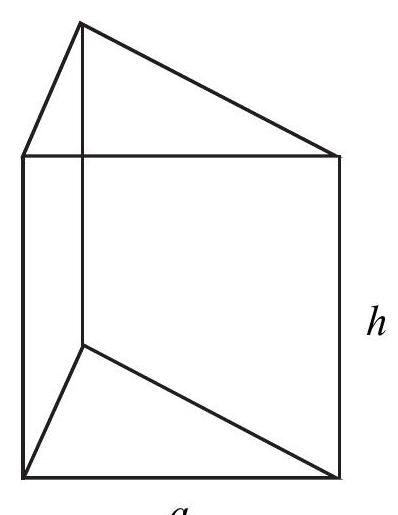
\includegraphics[max width=\textwidth, center]{2025_02_07_d712b9a47aa2c64928dbg-50}\\
$a$\\
Przyjmijmy oznaczenia jak na rysunku: $a$ - krawędź podstawy, $h$ - wysokość graniastosłupa. Objętość graniastosłupa prawidłowego trójkątnego o krawędzi podstawy $a$ i wysokości $h$ wyraża się wzorem:

$$
V=\frac{a^{2} \sqrt{3}}{4} \cdot h .
$$

Stąd otrzymujemy:

$$
2=\frac{a^{2} \sqrt{3}}{4} \cdot h .
$$

Zatem $h=\frac{8}{a^{2} \sqrt{3}}$.\\
Pole powierzchni całkowitej graniastosłupa prawidłowego trójkątnego o krawędzi podstawy $a$ i wysokości $h$ jest równe:

$$
P_{c}=2 \cdot \frac{a^{2} \sqrt{3}}{4}+3 \cdot a \cdot \frac{8}{a^{2} \sqrt{3}} .
$$

Stąd po podstawieniu $h$ i przekształceniach otrzymujemy:

$$
P_{c}=2 \cdot \frac{a^{2} \sqrt{3}}{4}+3 \cdot a \cdot \frac{8}{a^{2} \sqrt{3}}=\frac{a^{2} \sqrt{3}}{2}+\frac{24}{a \sqrt{3}}=\frac{a^{2} \sqrt{3}}{2}+\frac{8 \sqrt{3}}{a} .
$$

Z geometrycznych warunków zadania wynika, że $a \in(0 ;+\infty)$.\\
Zapiszmy pole powierzchni całkowitej graniastosłupa prawidłowego trójkątnego jako funkcję $f$ zmiennej $a$ :

$$
P_{c}=f(a)=\frac{a^{2} \sqrt{3}}{2}+\frac{8 \sqrt{3}}{a}=\frac{a^{3} \sqrt{3}+16 \sqrt{3}}{2 a}, \text { dla } a \in(0 ;+\infty) .
$$

Wyznaczamy wartość najmniejszą funkcji $f$ w przedziale $(0 ;+\infty)$.\\
W tym celu obliczmy pochodną funkcji $f$ :

$$
f^{\prime}(a)=\frac{3 a^{2} \sqrt{3} \cdot 2 a-\left(a^{3} \sqrt{3}+16 \sqrt{3}\right) \cdot 2}{4 a^{2}}=\frac{4 a^{3} \sqrt{3}-32 \sqrt{3}}{4 a^{2}} .
$$

Szukamy miejsc zerowych pochodnej funkcji $f$ :

$$
\frac{4 a^{3} \sqrt{3}-32 \sqrt{3}}{4 a^{2}}=0
$$

Ustalamy, że $a=2$.\\
W przedziale $(0 ;+\infty)$ pochodna funkcji $f$ ma tylko jedno miejsce zerowe $a=2$.\\
Ponadto\\
$f^{\prime}(a)>0$ dla $a \in(2 ;+\infty)$ oraz $f^{\prime}(a)<0$ dla $a \in(0 ; 2)$.

Wynika stąd, że dla $a=2$ funkcja $f$ ma minimum lokalne, które jest jednocześnie najmniejszą wartością funkcji $f$ w przedziale $(0,+\infty)$, ponieważ funkcja $f$ w przedziale $\langle 2,+\infty)$ jest rosnąca, a w przedziale $(0,2\rangle$ funkcja $f$ jest malejąca.\\
Gdy $a=2$, to $h=\frac{8}{a^{2} \sqrt{3}}=\frac{8}{2^{2} \sqrt{3}}=\frac{2}{\sqrt{3}}=\frac{2 \sqrt{3}}{3}$.\\
Natomiast pole powierzchni całkowitej graniastosłupa jest równe:

$$
P c=\frac{a^{3} \sqrt{3}+16 \sqrt{3}}{2 a}=\frac{2^{3} \sqrt{3}+16 \sqrt{3}}{2 \cdot 2}=\frac{24 \sqrt{3}}{4}=6 \sqrt{3} .
$$

Odp.: Najmniejsze pole powierzchni całkowitej równe $6 \sqrt{3}$ ma graniastosłup prawidłowy trójkątny o wymiarach: krawędź podstawy $a=2$ i wysokość $h=\frac{2 \sqrt{3}}{3}$.


\end{document}